%# -*- coding:utf-8 -*-
\documentclass[12pt,aspectratio=169,mathserif]{beamer}		
%\documentclass[12pt,mathserif]{beamer}		
%设置为 Beamer 文档类型,设置字体为 10pt,长宽比为16:9,数学字体为 serif 风格
%\documentclass{beamer}

%%%%-----导入宏包-----%%%%
\usepackage{gdut}			%导入 GDUT 模板宏包
\usepackage{ctex}			%导入 ctex 宏包,添加中文支持
\usepackage{amsmath,amsfonts,amssymb,bm}   %导入数学公式所需宏包
\usepackage{color}			 %字体颜色支持
\usepackage{graphicx,hyperref,url}
\usepackage{metalogo}	% 非必须
\usepackage{multicol}
%% 上文引用的包可按实际情况自行增删
%%%%%%%%%%%%%%%%%%	


\beamertemplateballitem		%设置 Beamer 主题

%%%%------------------------%%%%%
\catcode`\。=\active         %或者=13
\newcommand{。}{.}				
%将正文中的“。”号转换为“.”。中文标点国家规范建议科技文献中的句号用圆点替代
%%%%%%%%%%%%%%%%%%%%%

% Bibliography settings 参考文献设置
\usepackage[style=ieee]{biblatex}
\setbeamertemplate{bibliography item}[text]


%\tiny\scriptsize\footnotesize\small\normalsize\large\Large\LARGE\huge\Huge   这些是调整字体大小的命令。

%%%%----首页信息设置----%%%%
\title[ 《铛铛支付》项目报告]{《铛铛支付》项目报告}
\subtitle{——一个面向企业的兼信息展示,用户管理等的多功能支付平台}			
%%%%----标题设置


\author[杜家楷]{
	\large 杜家楷 \\\medskip
	%{\small \url{xuezheng@mail2.gdut.edu.cn}} \\
	%{\small \url{http://www.gdut.edu.cn/}}
}
%%%%----个人信息设置

\institute[IOPP]{
	\normalsize 广东工业大学计算机学院 \\ 
	计算机类23(3)}
%%%%----机构信息

\date[Apr. 04 2024]{
	2024年4月29日}
%%%%----日期信息

\begin{document}
	
	%----------------------------------------------------------------------------------------
	%	TITLE PAGE
	%----------------------------------------------------------------------------------------
	
	\begin{frame}
		\titlepage
	\end{frame}				%生成标题页
	
	\begin{frame}{目录} % Table of contents slide, comment this block out to remove it
		%\tableofcontents % Throughout your presentation, if you choose to use \section{} and \subsection{} commands, these will automatically be printed on this slide as an overview of your presentation
		\tableofcontents[sectionstyle=show,subsectionstyle=show/shaded/hide,subsubsectionstyle=show/shaded/hide]
		
	\end{frame}
	
	\AtBeginSection[]
	{
		\begin{frame}
			\frametitle{目录}
			\tableofcontents[currentsection]
		\end{frame}
	}
	
	
	%----------------------------------------------------------------------------------------
	%	PRESENTATION SLIDES
	%----------------------------------------------------------------------------------------
	
	%------------------------------------------------
	\section{介绍}% Sections can be created in order to organize your presentation into discrete blocks, all sections and subsections are automatically printed in the table of contents as an overview of the talk
	%------------------------------------------------
	
	\begin{frame}
		\frametitle{介绍}
		
		% \begin{itemize}
			
			
			%   \item {编译方式}
			%     \begin{itemize}
				%     	\item  推荐使用 Overleaf
				%     	\item 使用 \XeLaTeX 编译
				%     \end{itemize}
			%   \item 请参考 \LaTeX 和 Beamer 用户文档 
			
			%   \item 行内数学公式示例 $\sin^2 \theta + \cos^2 \theta = 1$
			%   \item {行间数学公式示例 \begin{equation}
					%     y_{1}=\int \sin x\, {\rm d}x
					%   \end{equation}	 }   
			% \end{itemize}
		\begin{block}{}
			随着数字货币成为越来越多人的支付方式选择,一个安全高效,功能丰富的资金管理网站可以更好地满足用户的需求,可以让用户更好地管理自己的资金,确认资金明细。
			
		\end{block}
		
		\begin{block}{Dangpay}
			铛铛支付是一个面向企业的兼信息展示,用户管理等的多功能支付平台,为企业的数字化转型赋能。
		\end{block}
	\end{frame}
	
	\section{设计思路}
	
	
	
	\begin{frame}{设计思路}
		\framesubtitle{}
		
		
		\begin{itemize}
			
			\item 整体采用前后端分离架构设计,旨在实现系统的高可扩展性、灵活性和可维护性。前端采用响应式设计,能够适应不同设备和屏幕尺寸,提供用户友好的交互体验。后端采用分布式架构,各个组件之间通过API进行交互,实现了系统的松耦合和高内聚。
			
			\item 在支付平台的设计中,我们遵循了面向服务的架构(SOA)思想和MVC思想,各个业务模块之间通过服务接口进行交互,实现了系统的模块化和可重用性。
			
			\item 此外,我们还考虑到了系统的安全性和可靠性,采用了多种安全机制和故障恢复机制,确保了系统的稳定运行和数据安全。
			
		\end{itemize}
	\end{frame}
	
	
	
	\begin{frame}{技术选型}
		
		我的项目使用了以下技术栈:
		
		\textbf{}
		
		\begin{itemize}
			\item \textbf{Java Servlet}  HTTP Server
			\item \textbf{TiDB} 兼容mysql的数据库服务
			\item \textbf{Minio} 非结构化文件存储
			\item \textbf{Redis} 缓存和分布式锁
			\item \textbf{Kubernetes} 容器编排
		\end{itemize}
		
	\end{frame}
	
	%------------------------------------------------
	
	
	\section{项目功能}
	
	
	
	
	\begin{frame}
		\frametitle{总览}
		项目主要有主页,群组,钱包,私聊,交易记录,审计日志六个页面组成。
	\end{frame}
	
	
	\begin{frame}
		\frametitle{主页}
		
		主页有注册,登录,注销登录,以及登录之后查看和修改个人信息的功能。
		
		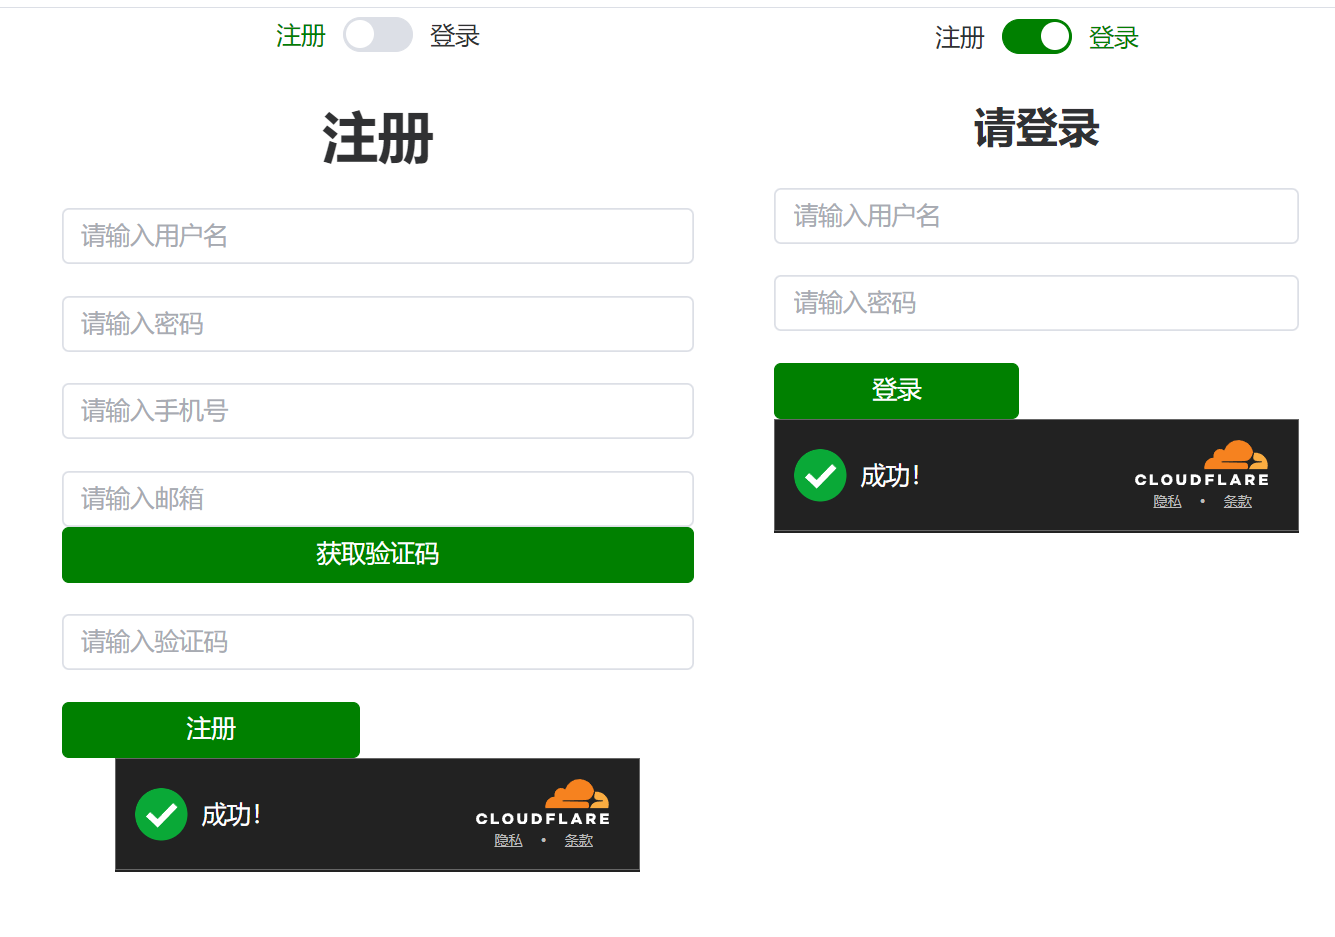
\includegraphics[width=0.8\textwidth]{assets/image-20240429120546182.png}
		
		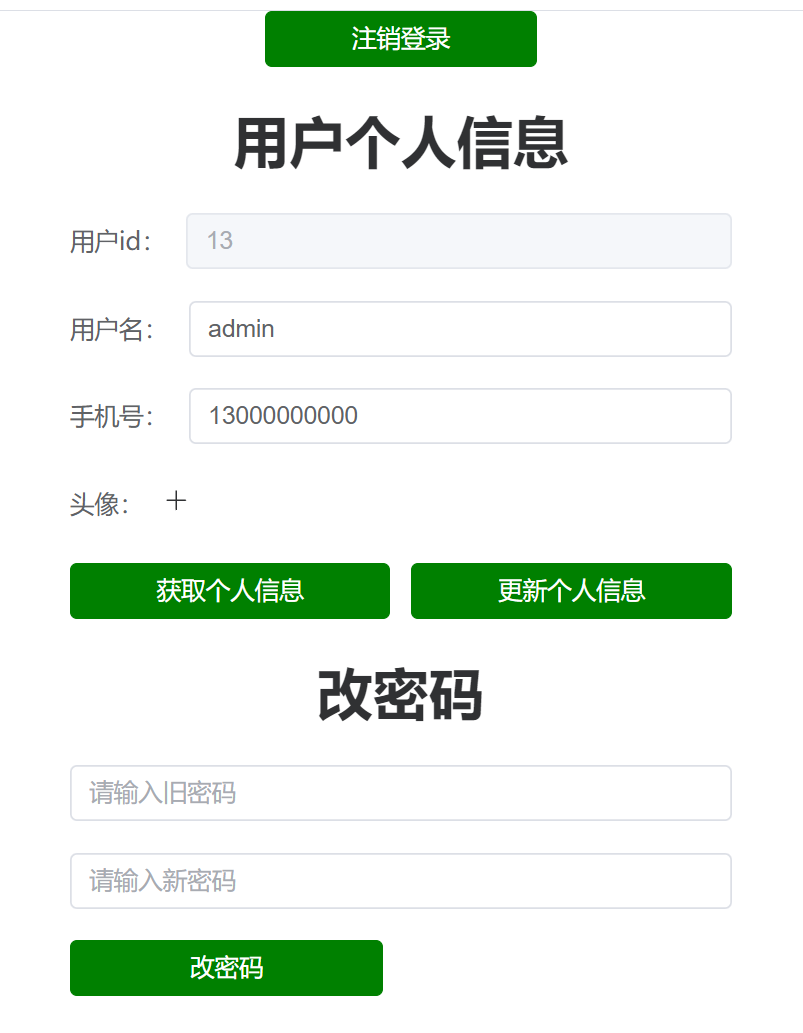
\includegraphics[width=0.8\textwidth]{assets/image-20240429120637515.png}
		
	\end{frame}
	
	
	\begin{frame}
		\frametitle{群组页面}
		
		有查看群组列表,创建群组和查看我的群组功能。
		
		创建群组将会向网站管理员发送申请,管理员审批通过即成功创建群组。
		
		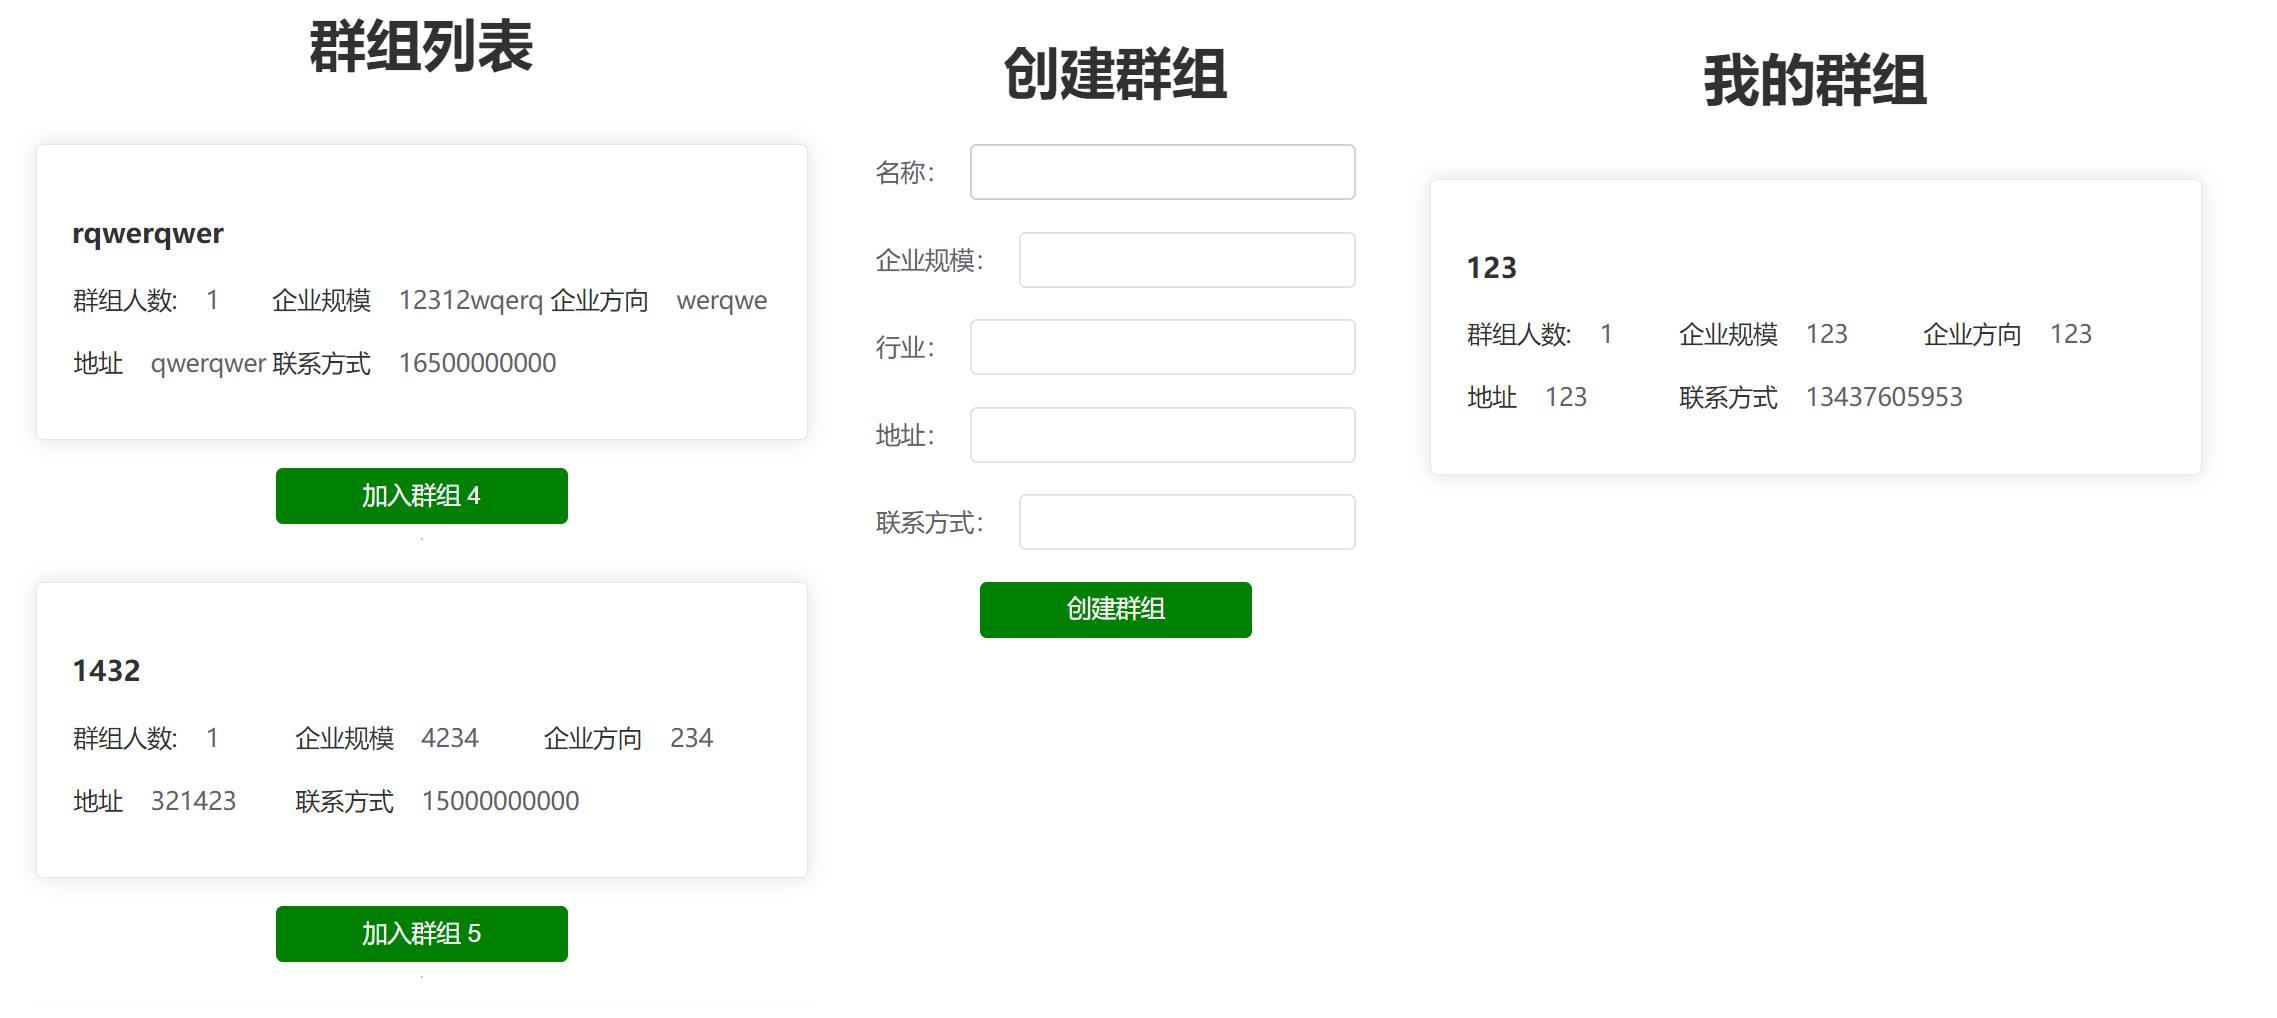
\includegraphics[width=0.8\textwidth]{assets/image-20240429120922179.png}
		
	\end{frame}
	
	
	\begin{frame}
		\frametitle{群组页面}
		
		\begin{minipage}{0.4\linewidth}
			网站管理员会比普通用户多出来可以封禁群组和解封群组的功能,被封禁的群组无法做任何操作,同时群组钱包会被冻结,无法进行交易,只能由群组管理员向网站管理员申请解封。
		\end{minipage}\hspace{0.3cm}
		\begin{minipage}{0.45\linewidth}
			\begin{figure}[h]
				\centering
				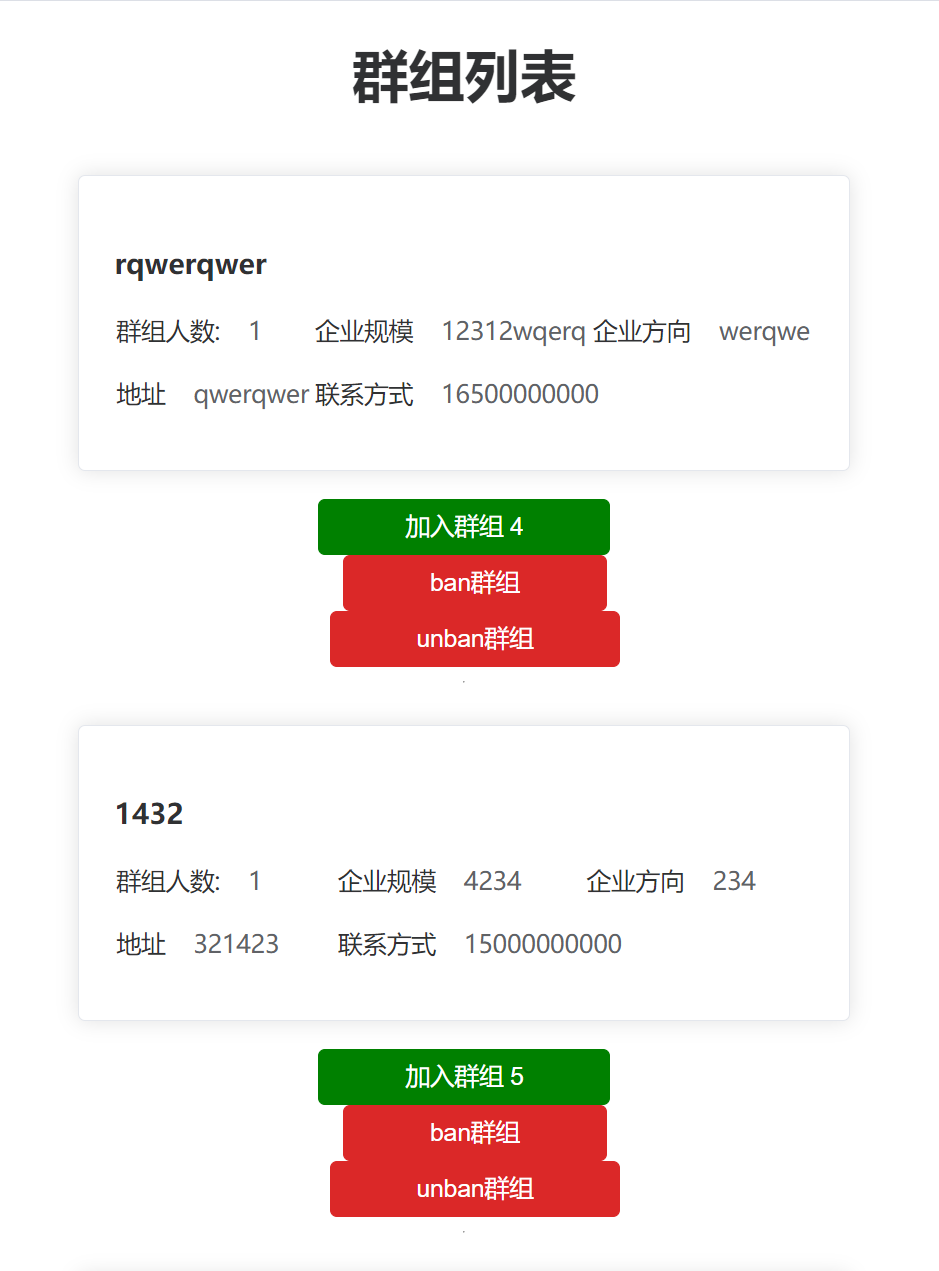
\includegraphics[height=\textheight]{assets/image-20240429131202427.png}
			\end{figure}
		\end{minipage}%\hspace{0.1cm}
		
	\end{frame}
	
	
	\begin{frame}
		\frametitle{群组详细页面}
		
		
		\begin{minipage}{0.4\linewidth}
			用户可以查看自己的群组的详细信息
		\end{minipage}\hspace{0.3cm}
		\begin{minipage}{0.45\linewidth}
			\begin{figure}[h]
				\centering
				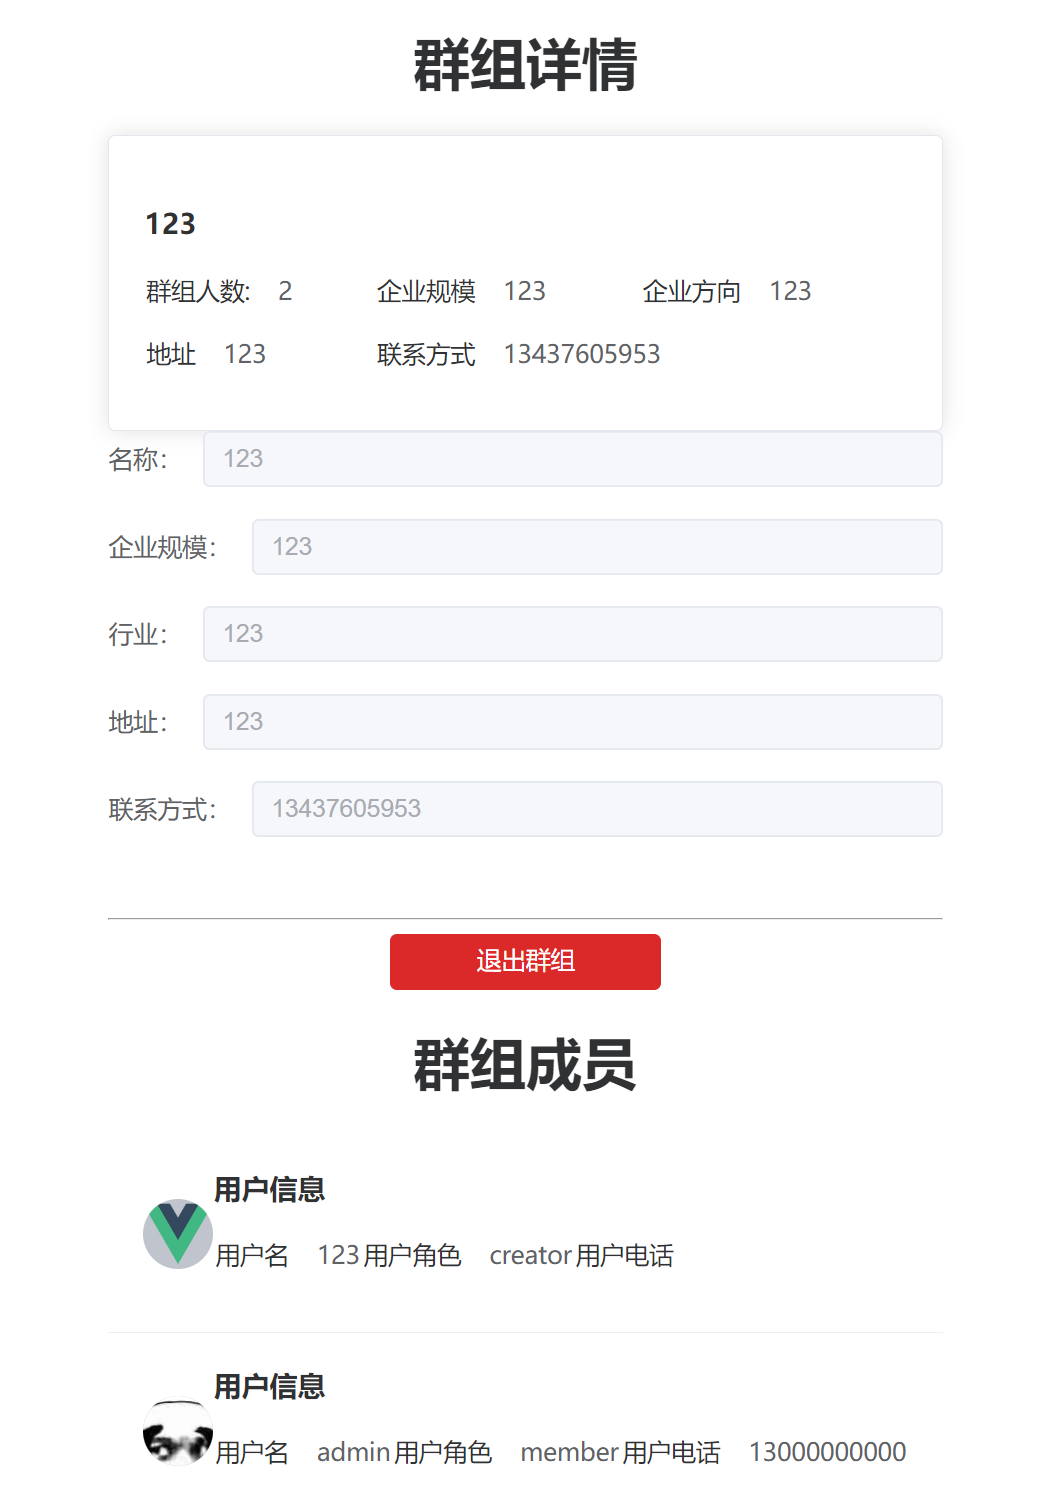
\includegraphics[height=\textheight]{assets/image-20240429122236442.png}
				
			\end{figure}
		\end{minipage}%\hspace{0.1cm}
		
	\end{frame}
	
	
	
	\begin{frame}
		\frametitle{群组详细页面}
		\begin{minipage}{0.4\linewidth}
			群组管理员会比普通的群组成员多出管理方面的功能
		\end{minipage}
		%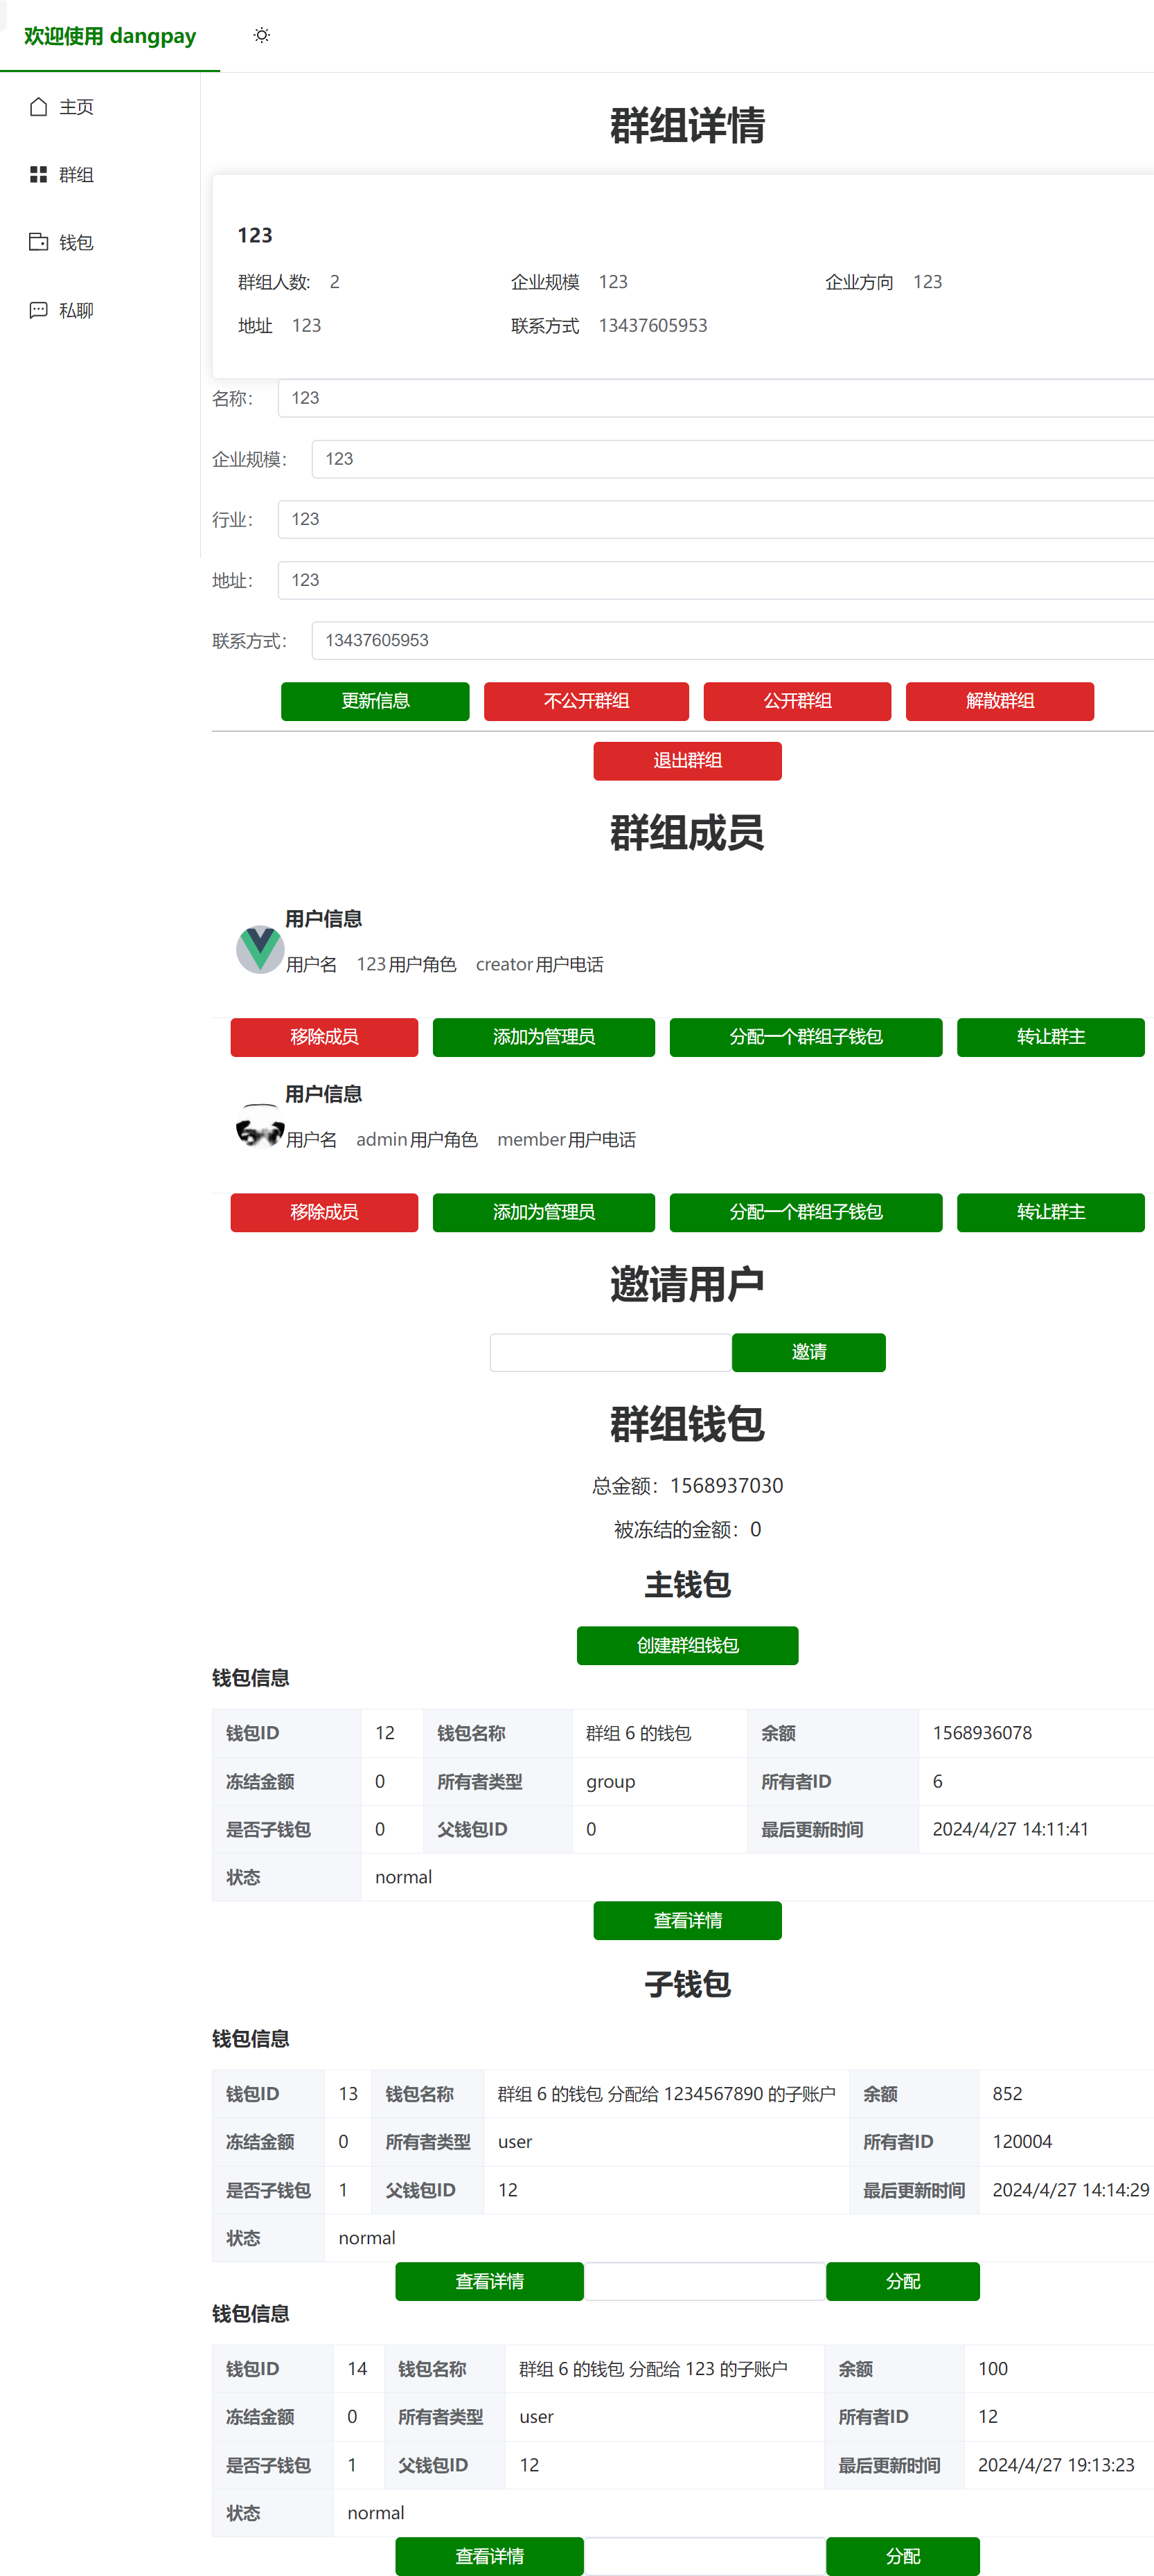
\includegraphics[width=0.4\textwidth]{assets/dangpay.99.suyiiyii.top_ (1)_1.png}
		\hspace{0.3cm}
		\begin{minipage}{0.45\linewidth}
			\begin{figure}[h]
				\centering
				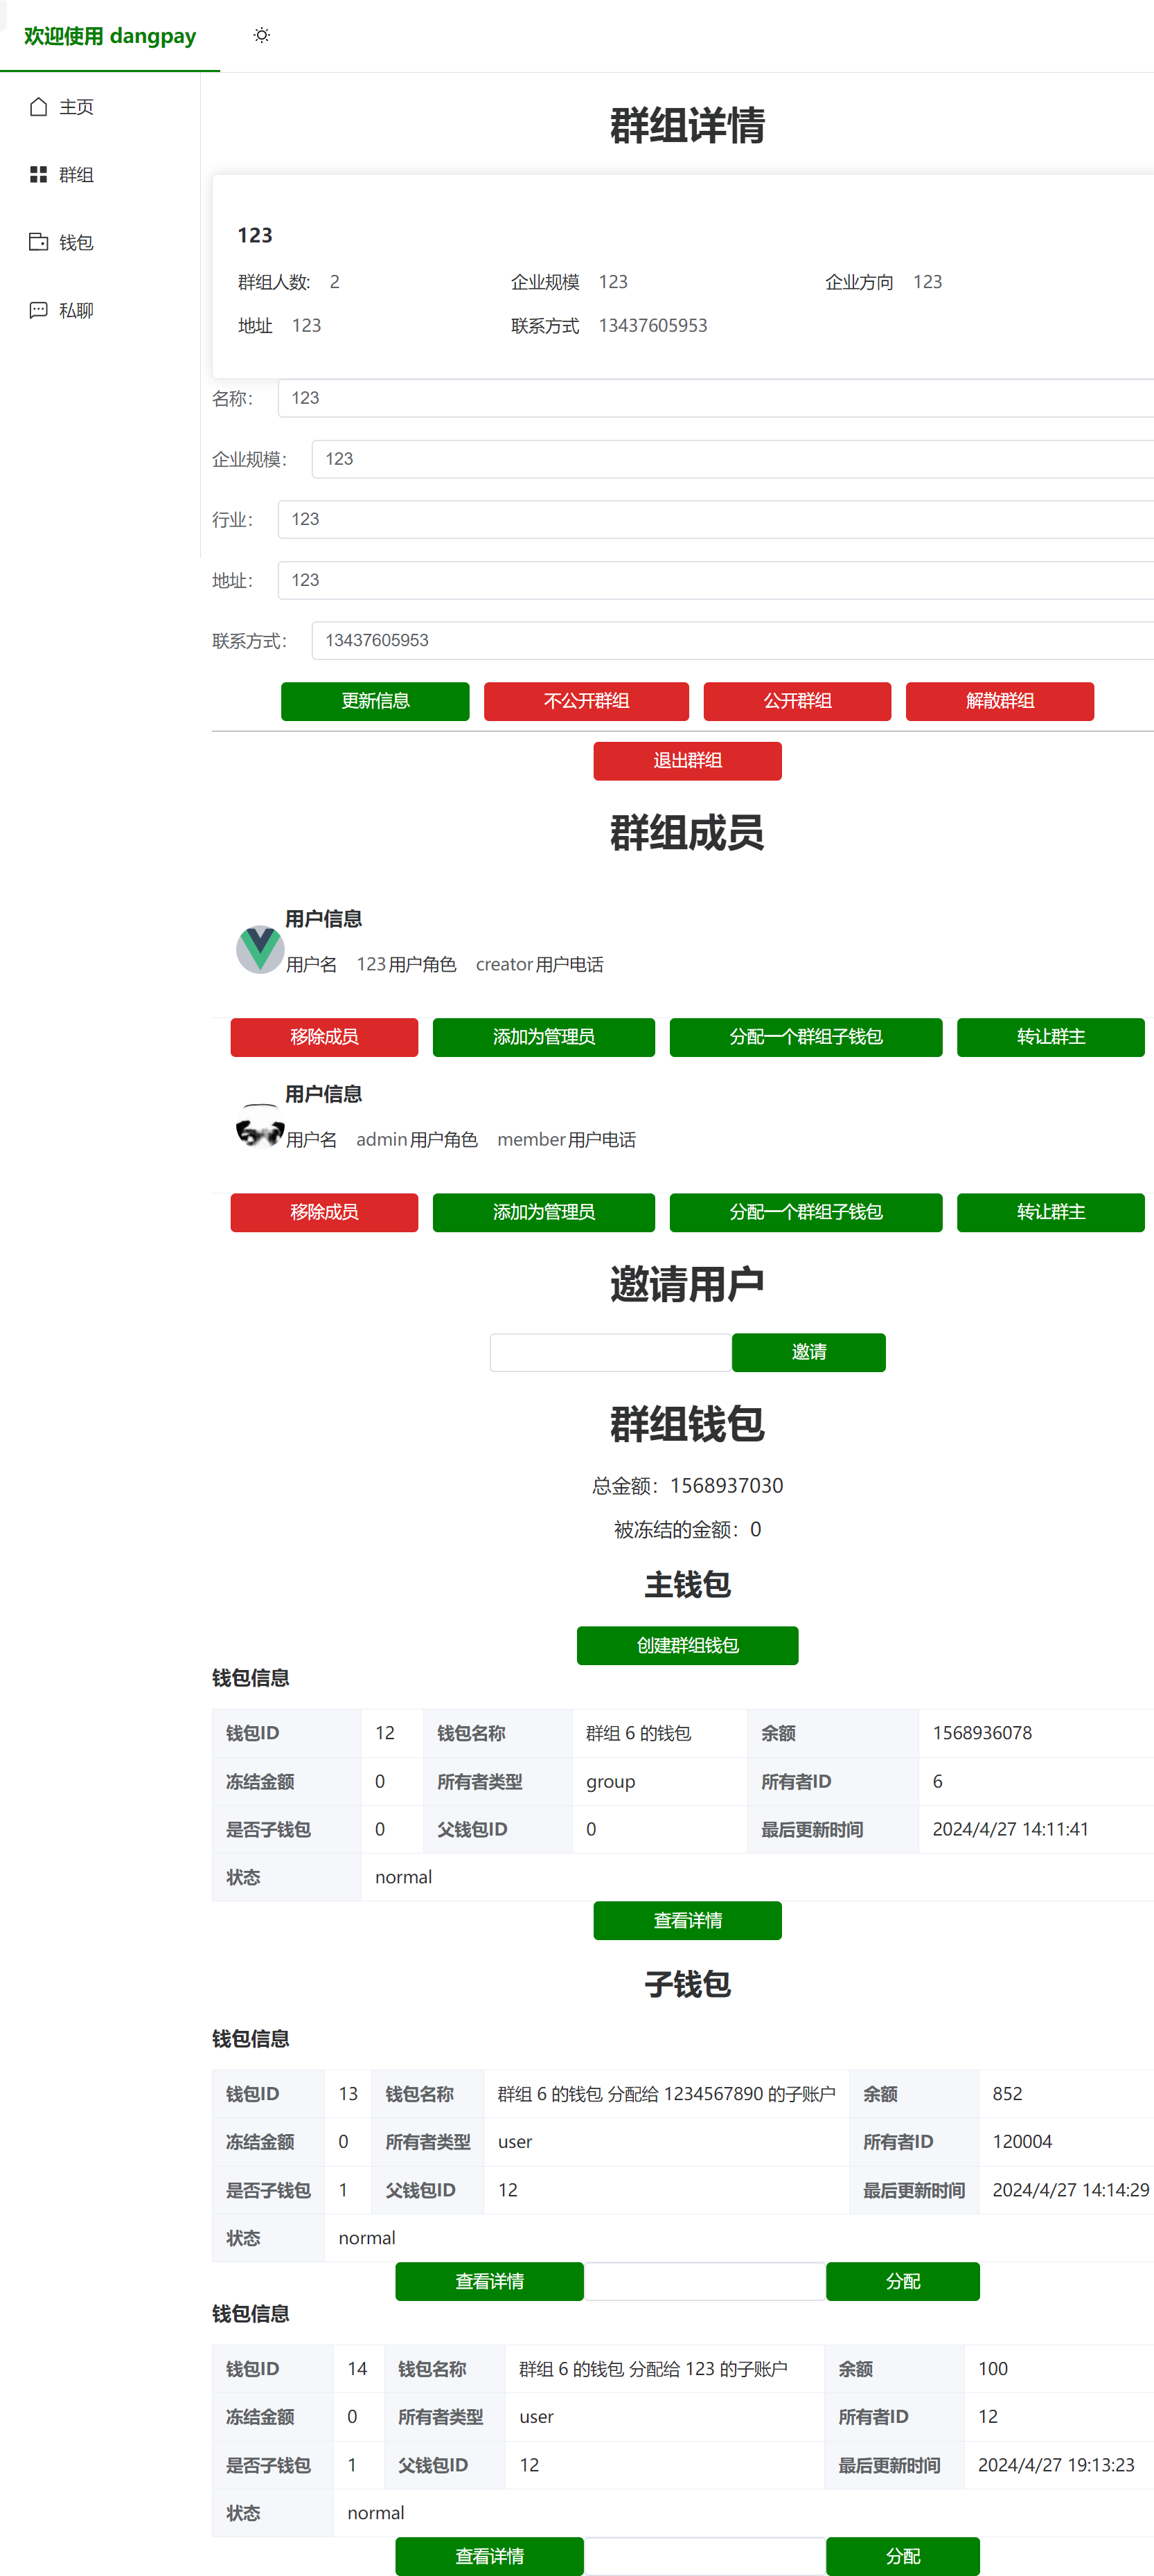
\includegraphics[height=\textheight]{assets/dangpay.99.suyiiyii.top_ (1)_1.png}
			\end{figure}
		\end{minipage}%\hspace{0.1cm}
	\end{frame}
	
	\begin{frame}
		\frametitle{钱包页面}
		群组的钱包系统分为群组主钱包和群组子钱包,主钱包归属于群组,不属于任何个人,无法使用群组主钱包直接对外进行交易。群组管理员可以给群组成员分配群组子钱包,子钱包归属于个人,和个人钱包一样,可以进行任何交易,同时可以接受群组主钱包分配和收回资金。如果群组管理员希望给其他成员分配资金,则可以给对应的群组子钱包转钱,然后讲自己的子钱包的钱转移到群组主钱包里,然后再用群组主钱包划分资金给需要分配的用户的群组子钱包。
		
	\end{frame}
	
	\begin{frame}
		\frametitle{钱包页面}
		\begin{minipage}{0.4\linewidth}
			钱包界面可以看到钱包的详细信息,可以生成收款二维码,可以扫描其他用户提供的收款二维码,可以查看该钱包的交易记录
		\end{minipage}
		\hspace{0.3cm}
		\begin{minipage}{0.45\linewidth}
			\begin{figure}[h]
				\centering
				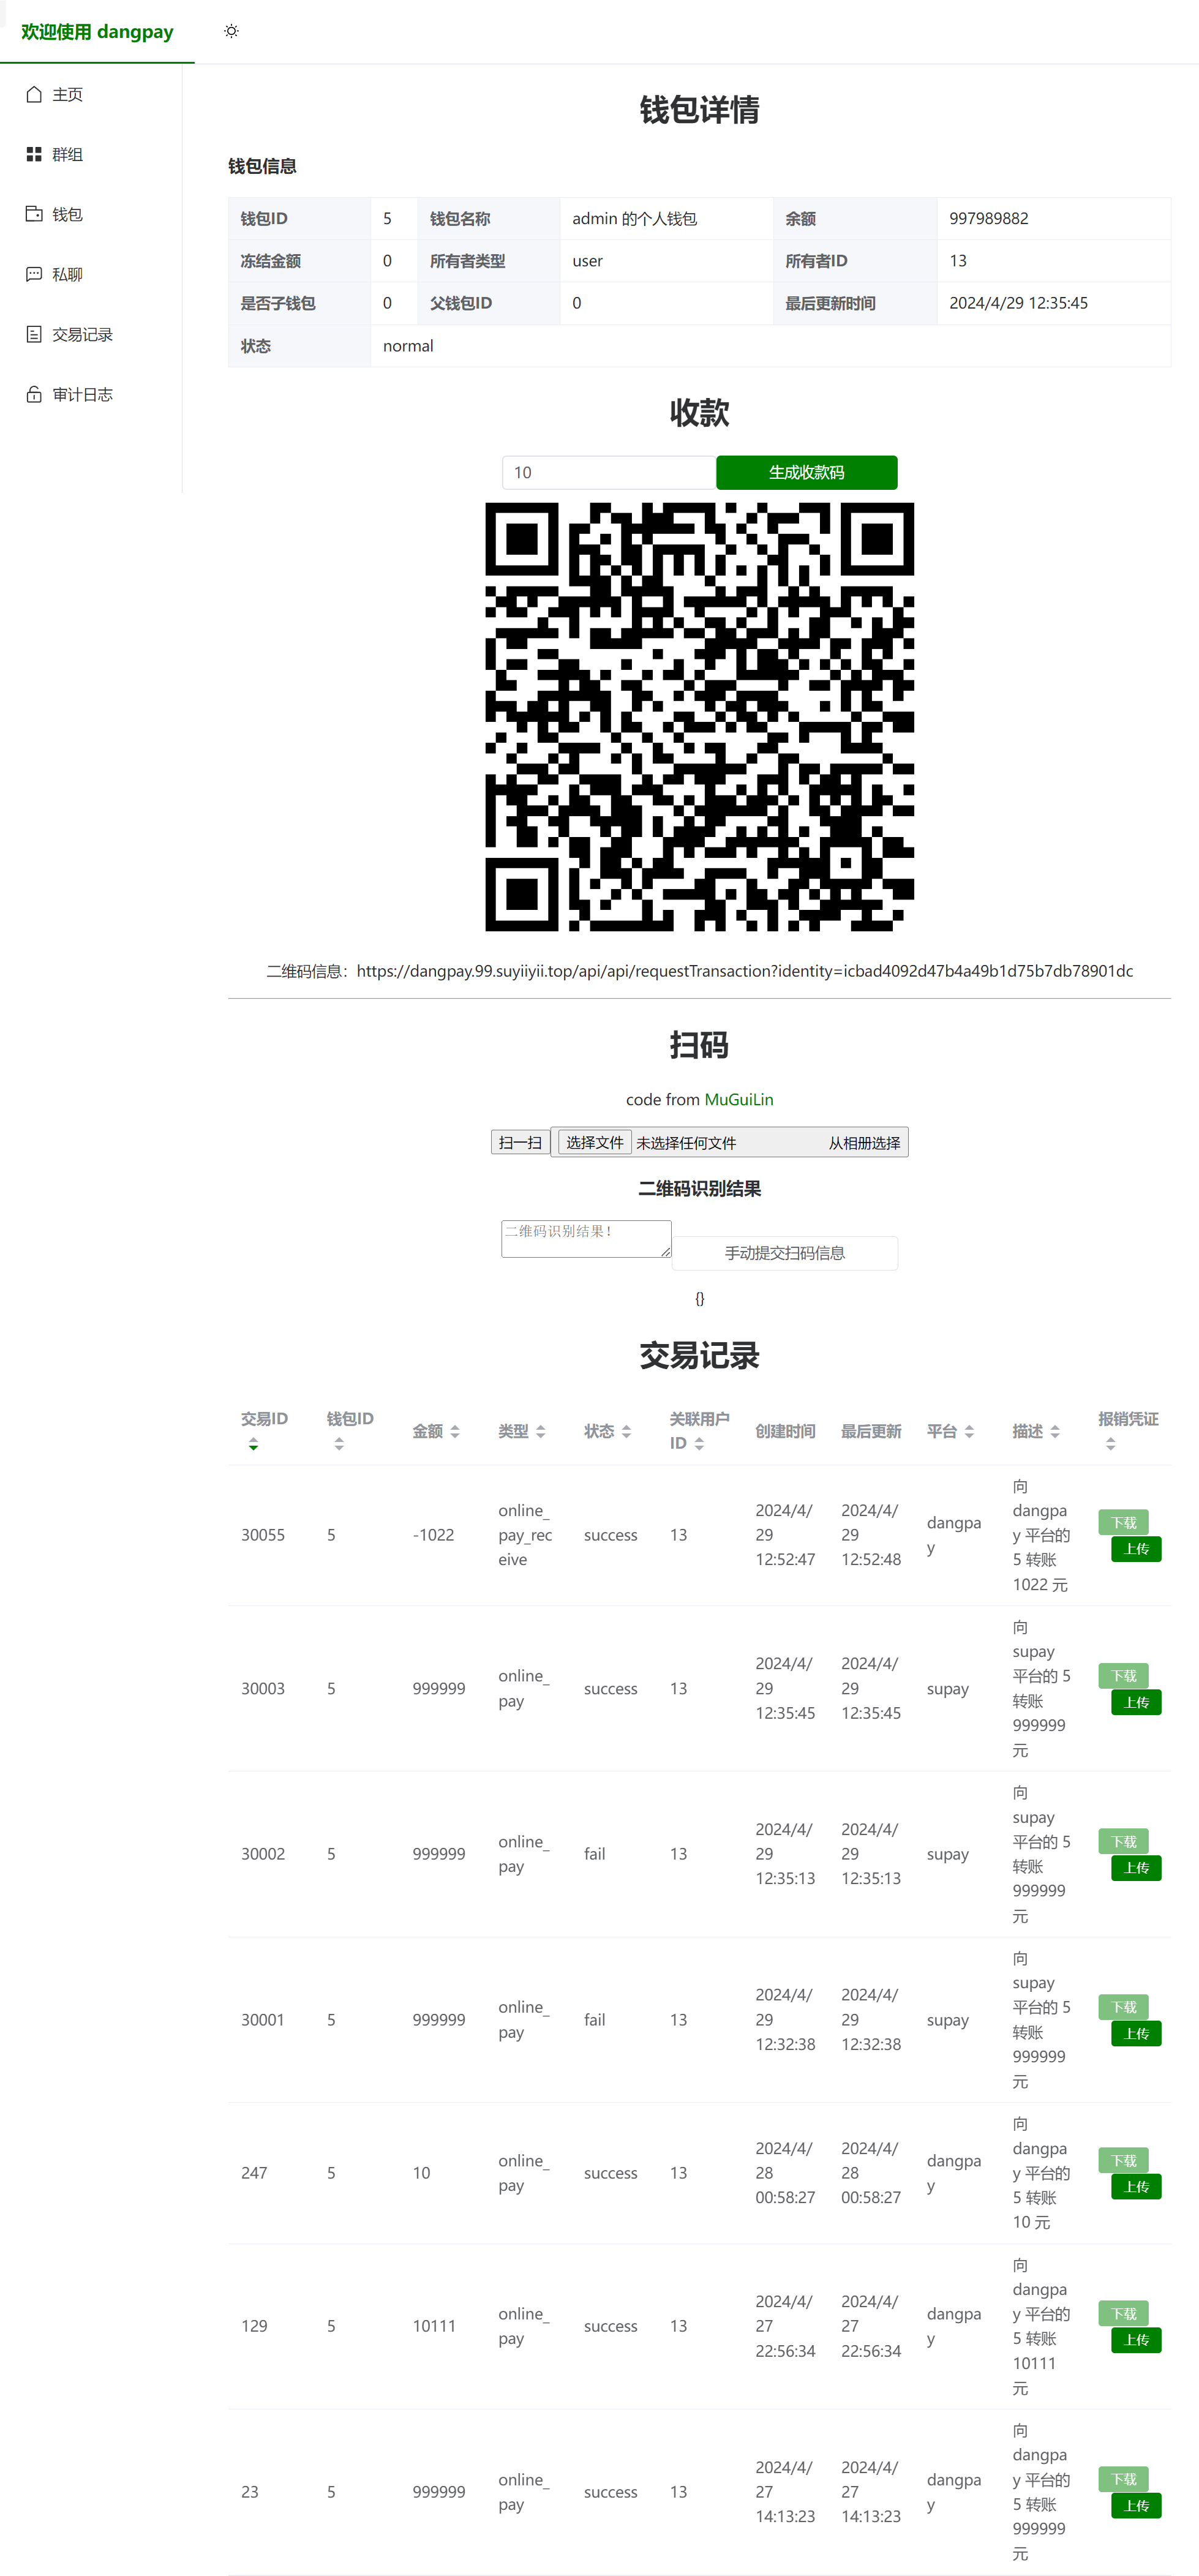
\includegraphics[height=\textheight]{assets/dangpay.99.suyiiyii.top_.png}
			\end{figure}
		\end{minipage}%\hspace{0.1cm}
		
	\end{frame}
	
	
	
	\begin{frame}
		\frametitle{私聊页面}
		用户可以在这里接收和处理系统通知,和其他用户以及群组内聊天
		\begin{minipage}{0.55\linewidth}
			\begin{figure}[h]
				\centering
				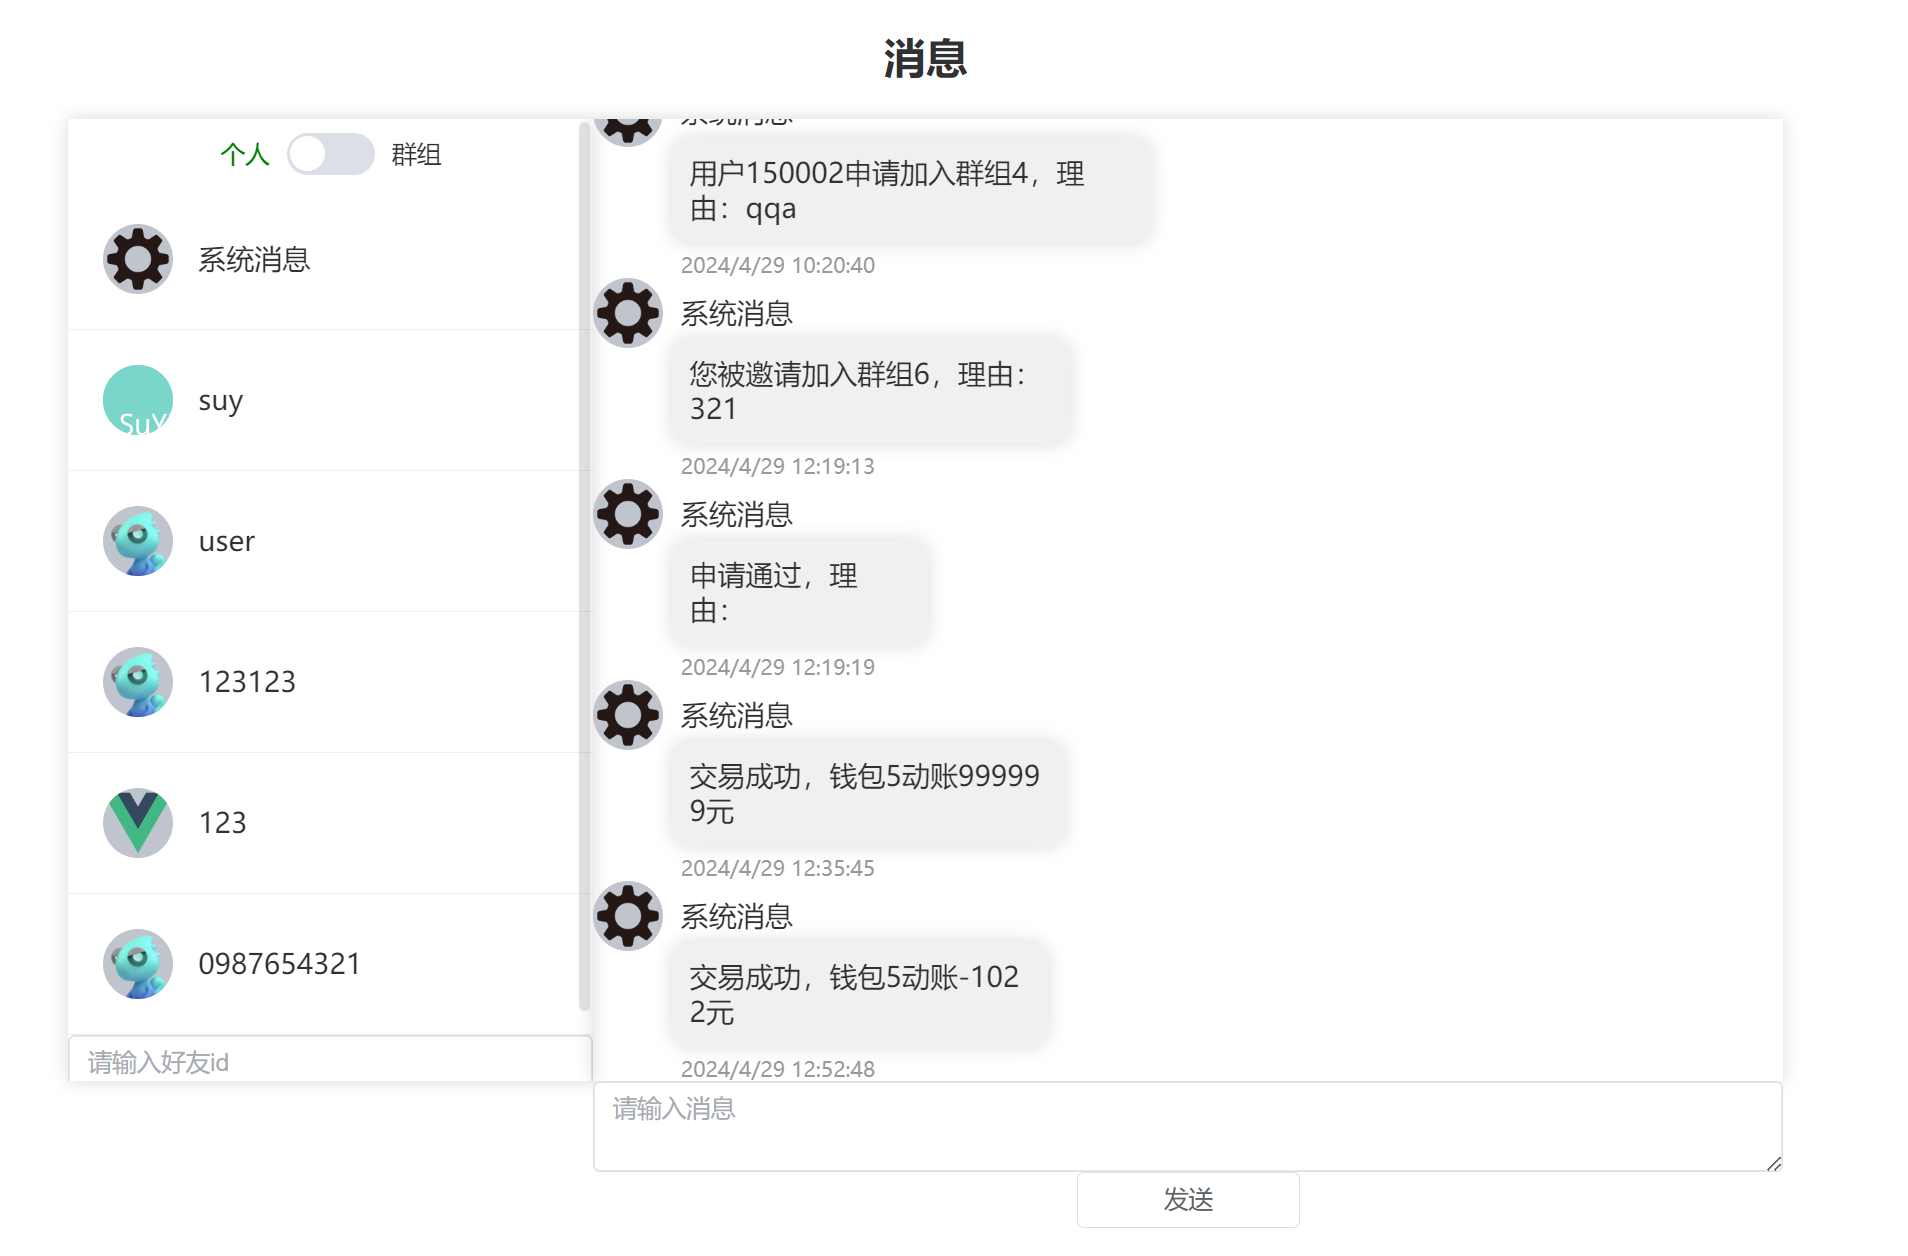
\includegraphics[height=\textheight]{assets/image-20240429125550801.png}
				
			\end{figure}
		\end{minipage}%\hspace{0.1cm}
		
		
	\end{frame}
	
	
	\begin{frame}
		\frametitle{全局交易记录}
		管理员可以在这个页面看到站内的所有交易记录,便于监管。
		
		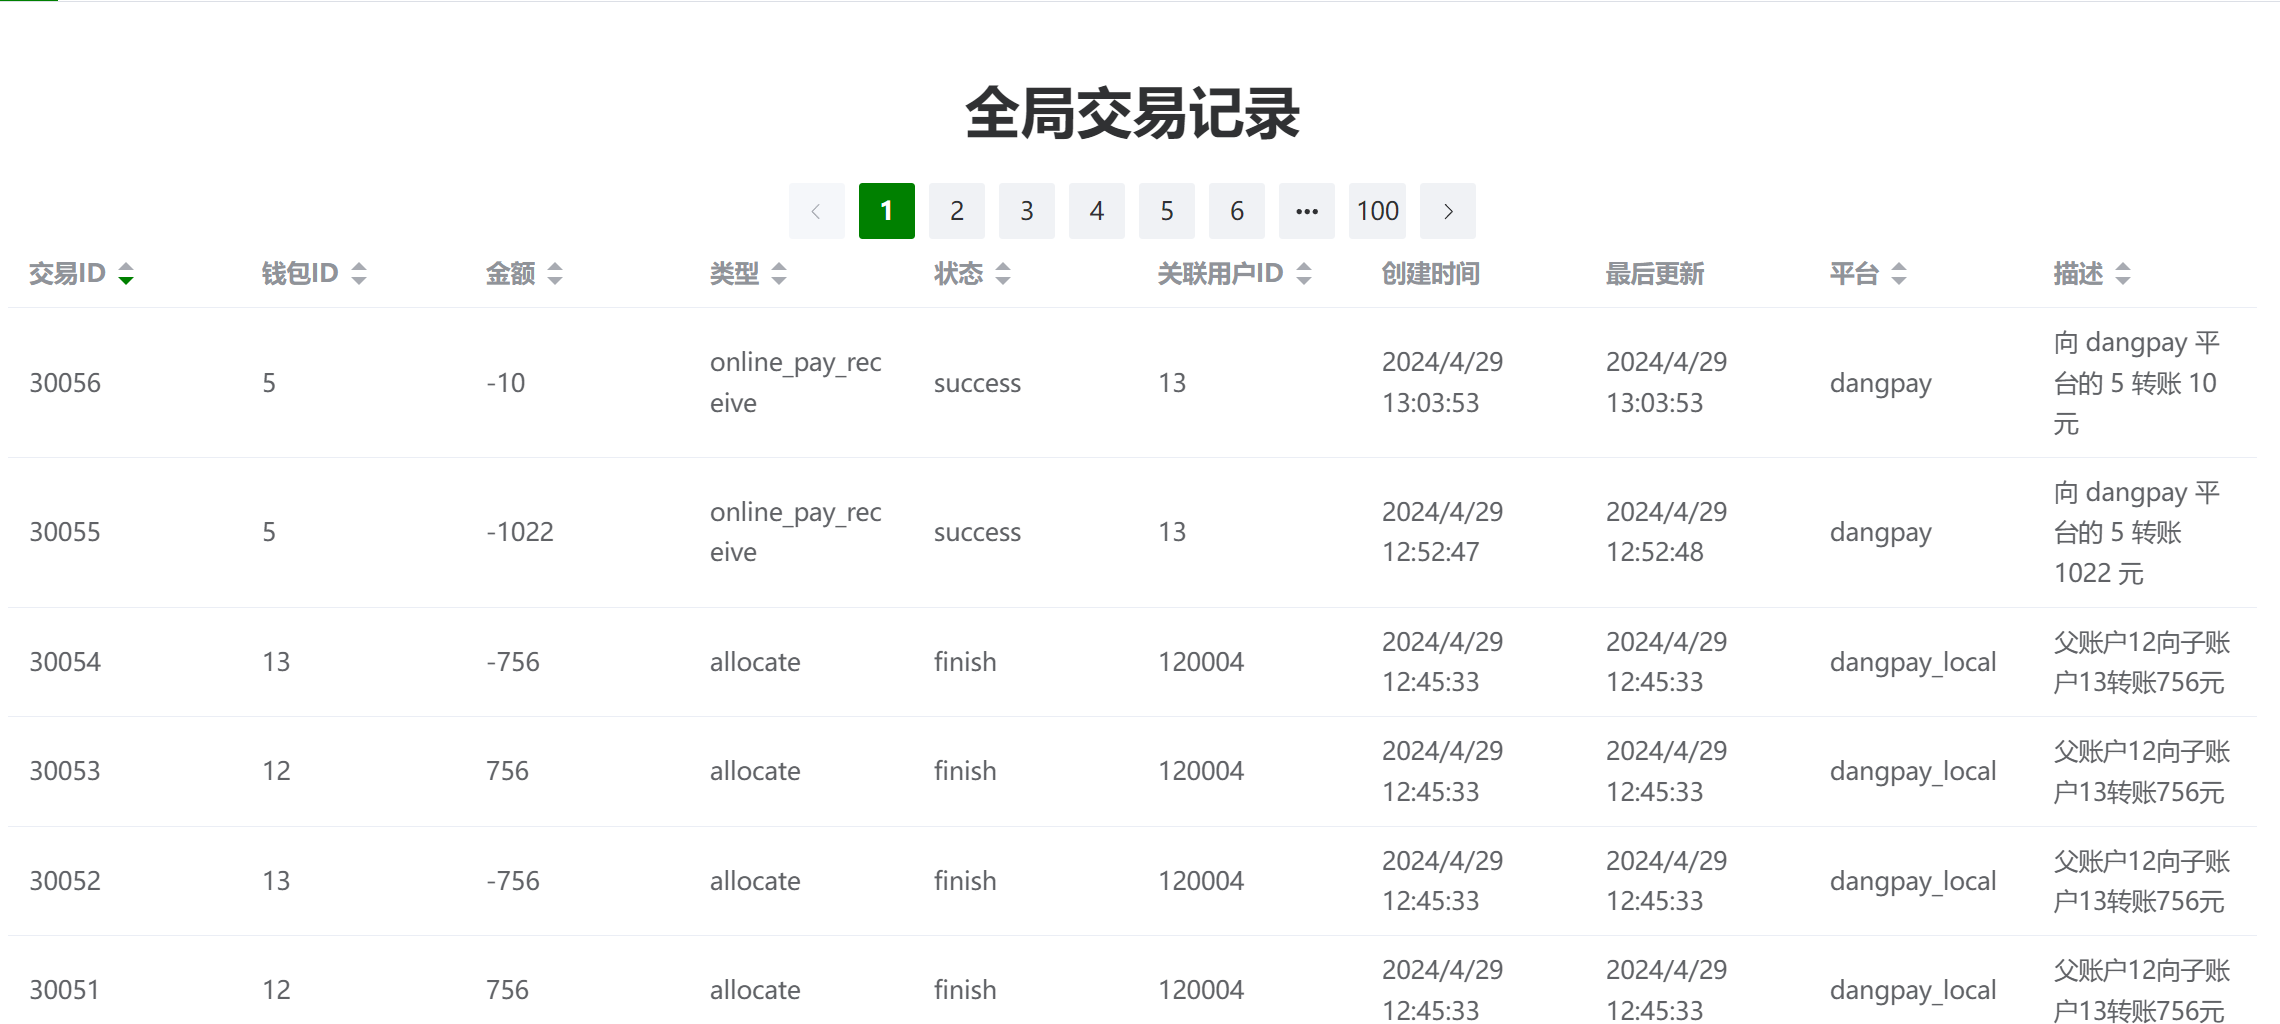
\includegraphics[width=0.8\textwidth]{assets/image-20240429130439225.png}
		
	\end{frame}
	
	
	\begin{frame}
		\frametitle{审计日志}
		管理员可以查看全站的审计日志,便于查找恶意用户。
		
		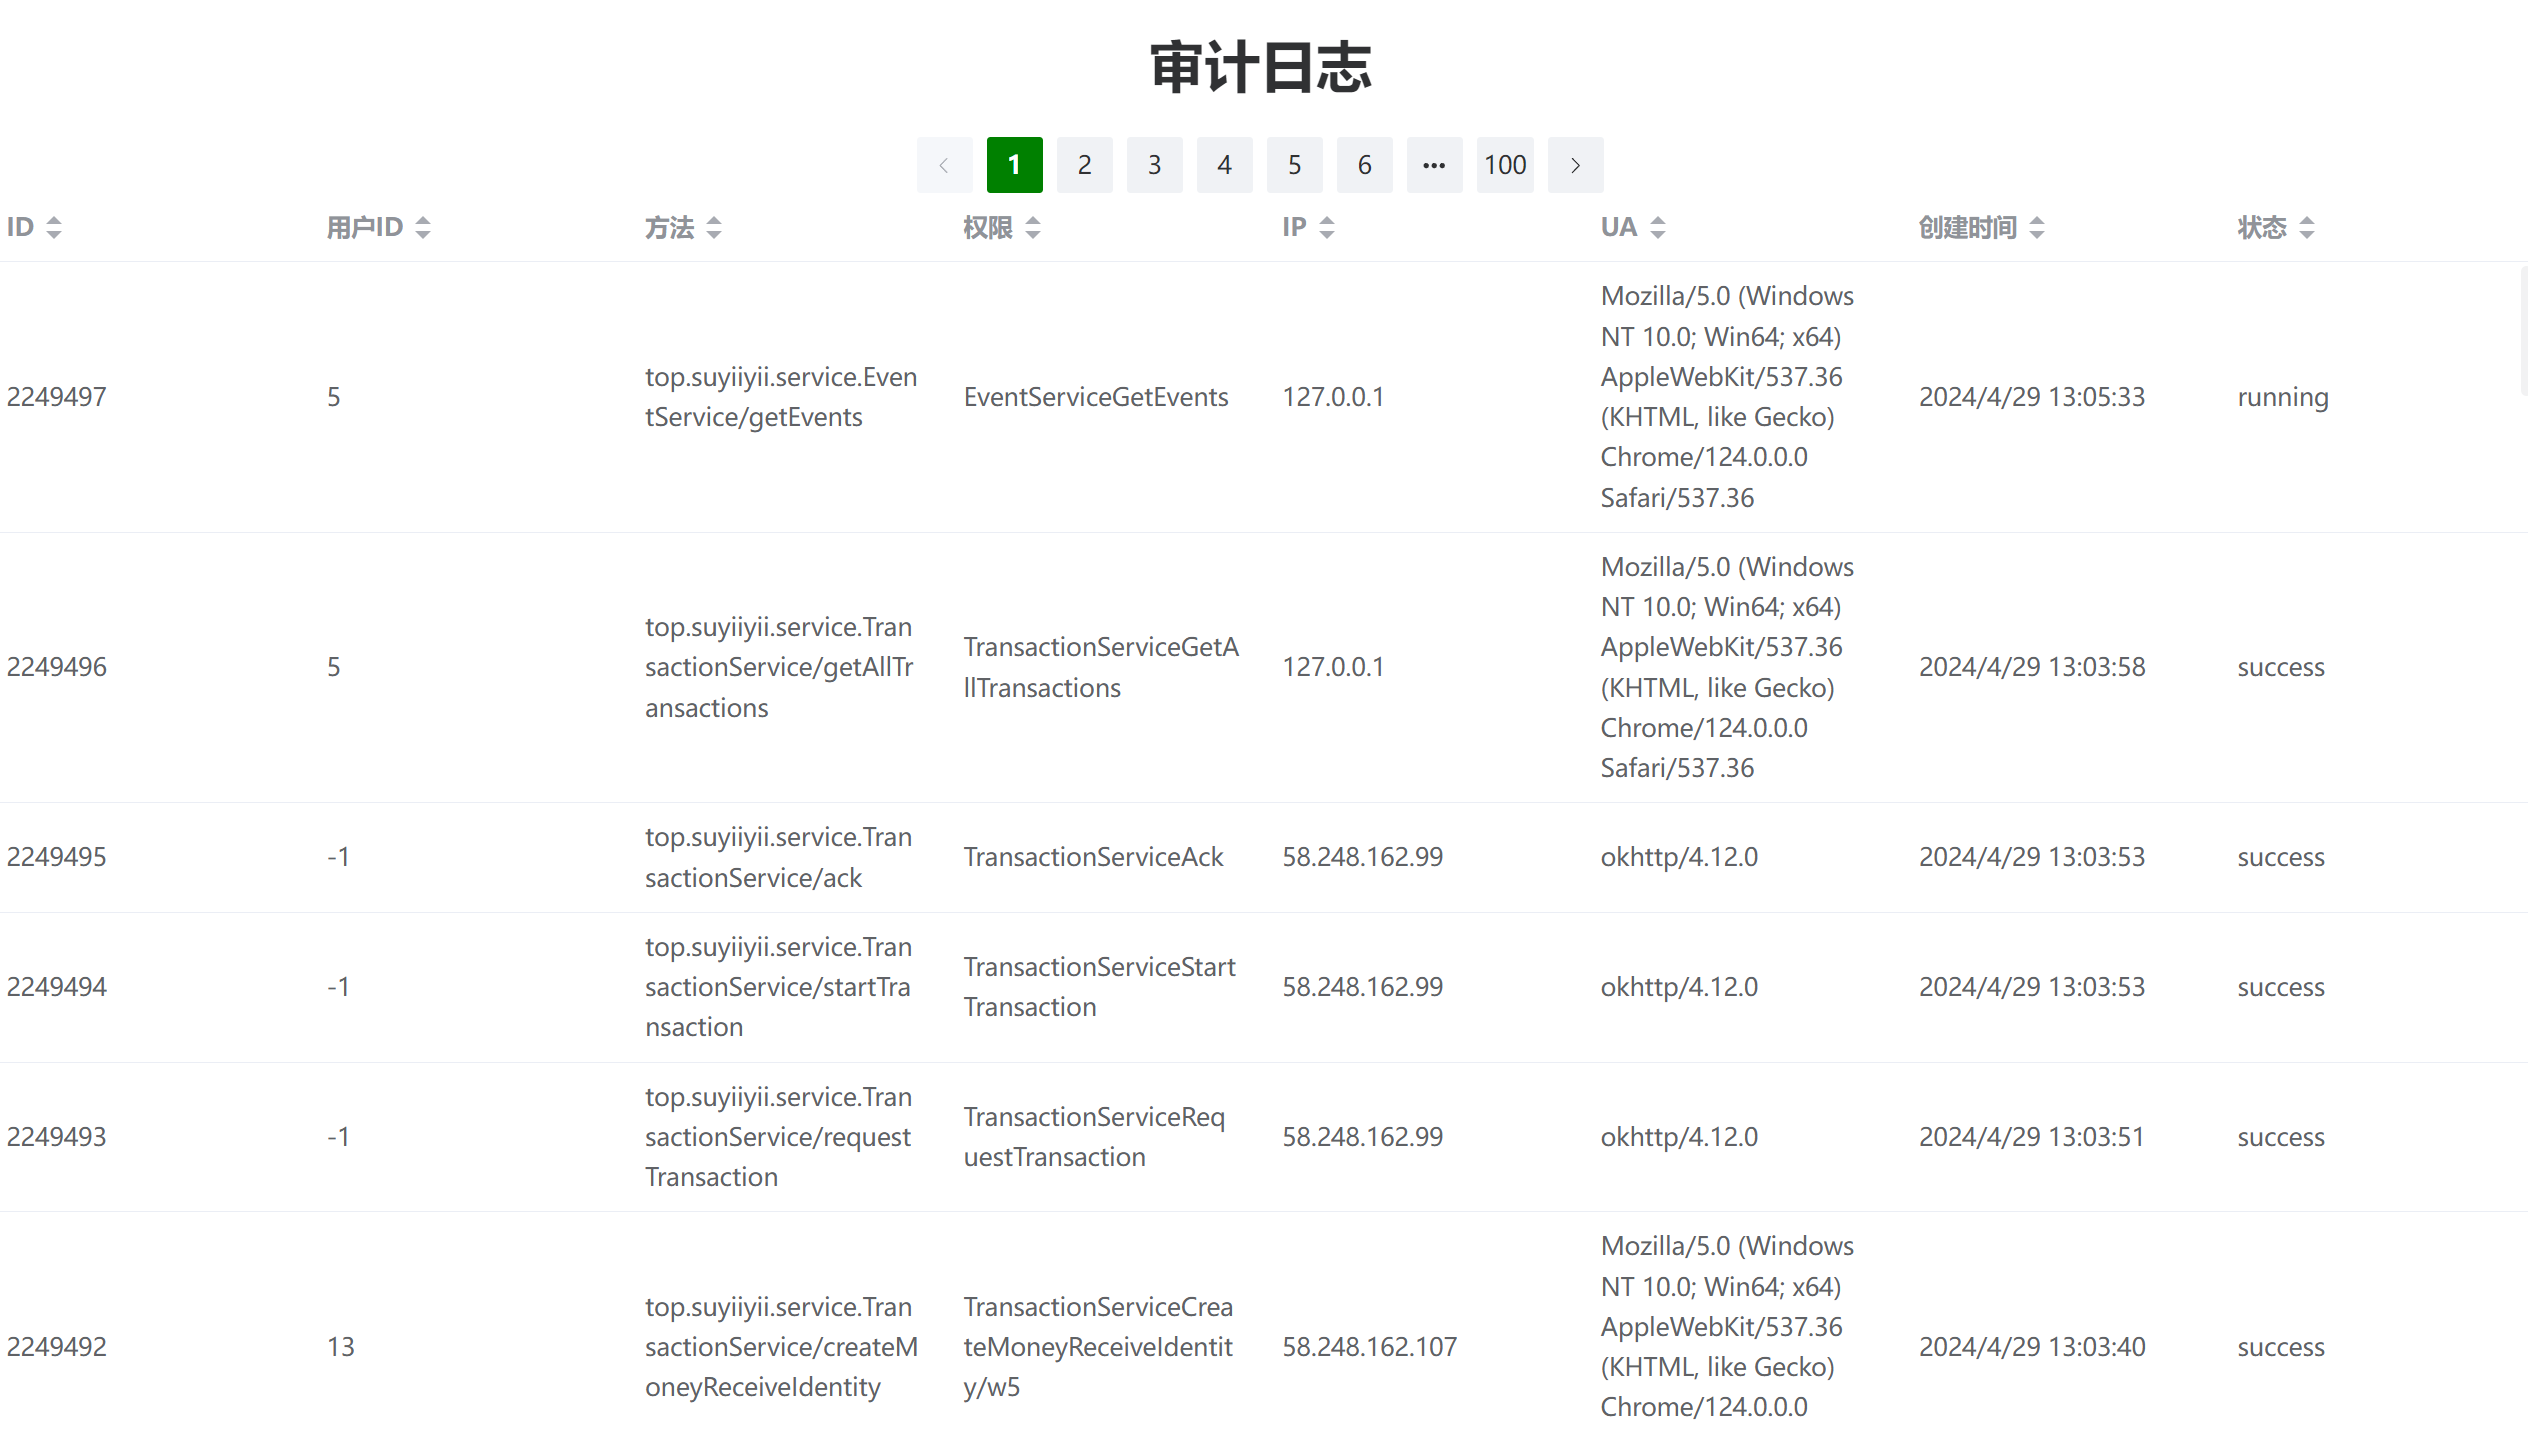
\includegraphics[width=0.8\textwidth]{assets/image-20240429130553723.png}
		
	\end{frame}
	


\section{项目代码亮点}


\begin{frame}{连接池}



  自己实现了jdbc的连接池,可以适配不同的数据库驱动,通过多线程实现高效的连接分配和收回操作,大大提高了连接的复用率,加速数据库操作,同时为orm框架的完成奠定基础。

\end{frame}



\begin{frame}{ORM}

  \begin{minipage}{0.4\linewidth}
    自己实现了一个简单的orm框架,具有自动根据实体类创建对应的数据库表,语义化的增删差改操作,批量插入对象,自动追踪被修改的元素并自动更新到数据库等功能。语句的执行起和查询条件的构造器使用回调函数实现了分离,并且支持链式调用,扩展性强。使用简单的java对象操作即可实现操作数据库,大大的提高了开发的效率。
  \end{minipage}\hspace{0.3cm}
  \begin{minipage}{0.45\linewidth}
    \begin{figure}[h]
      \centering
      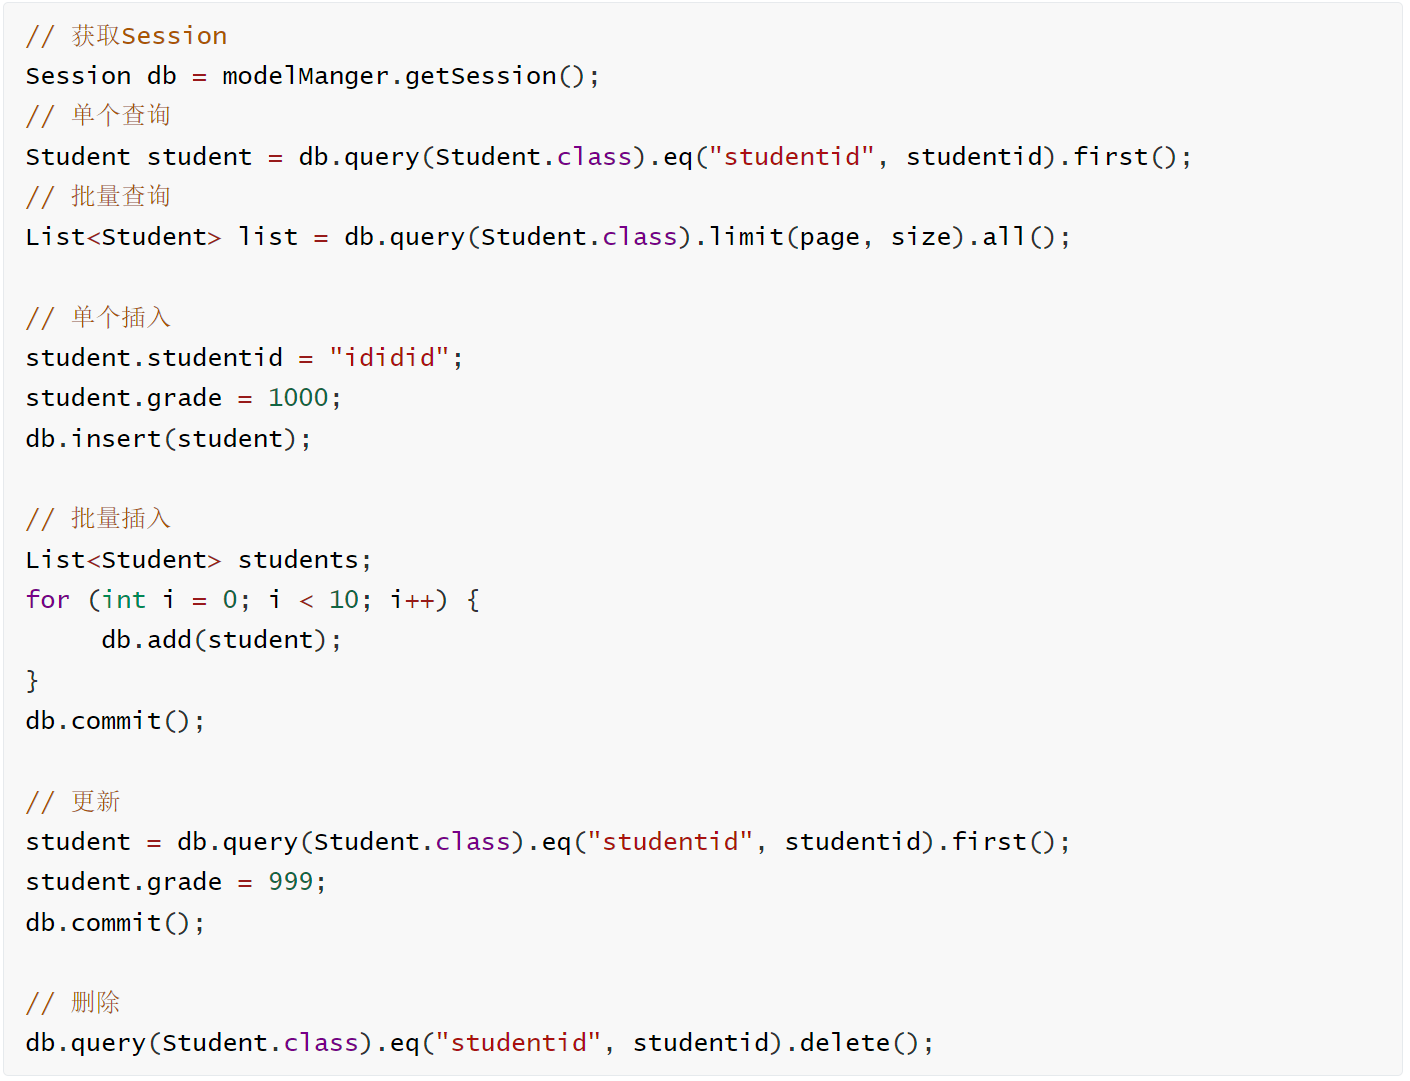
\includegraphics[height=\textheight]{assets/Snipaste_2024-04-29_15-32-40.png}

    \end{figure}
  \end{minipage}%\hspace{0.1cm}


\end{frame}

\begin{frame}{ORM架构图}


  \begin{minipage}{0.45\linewidth}
    \begin{figure}[h]
      \centering

      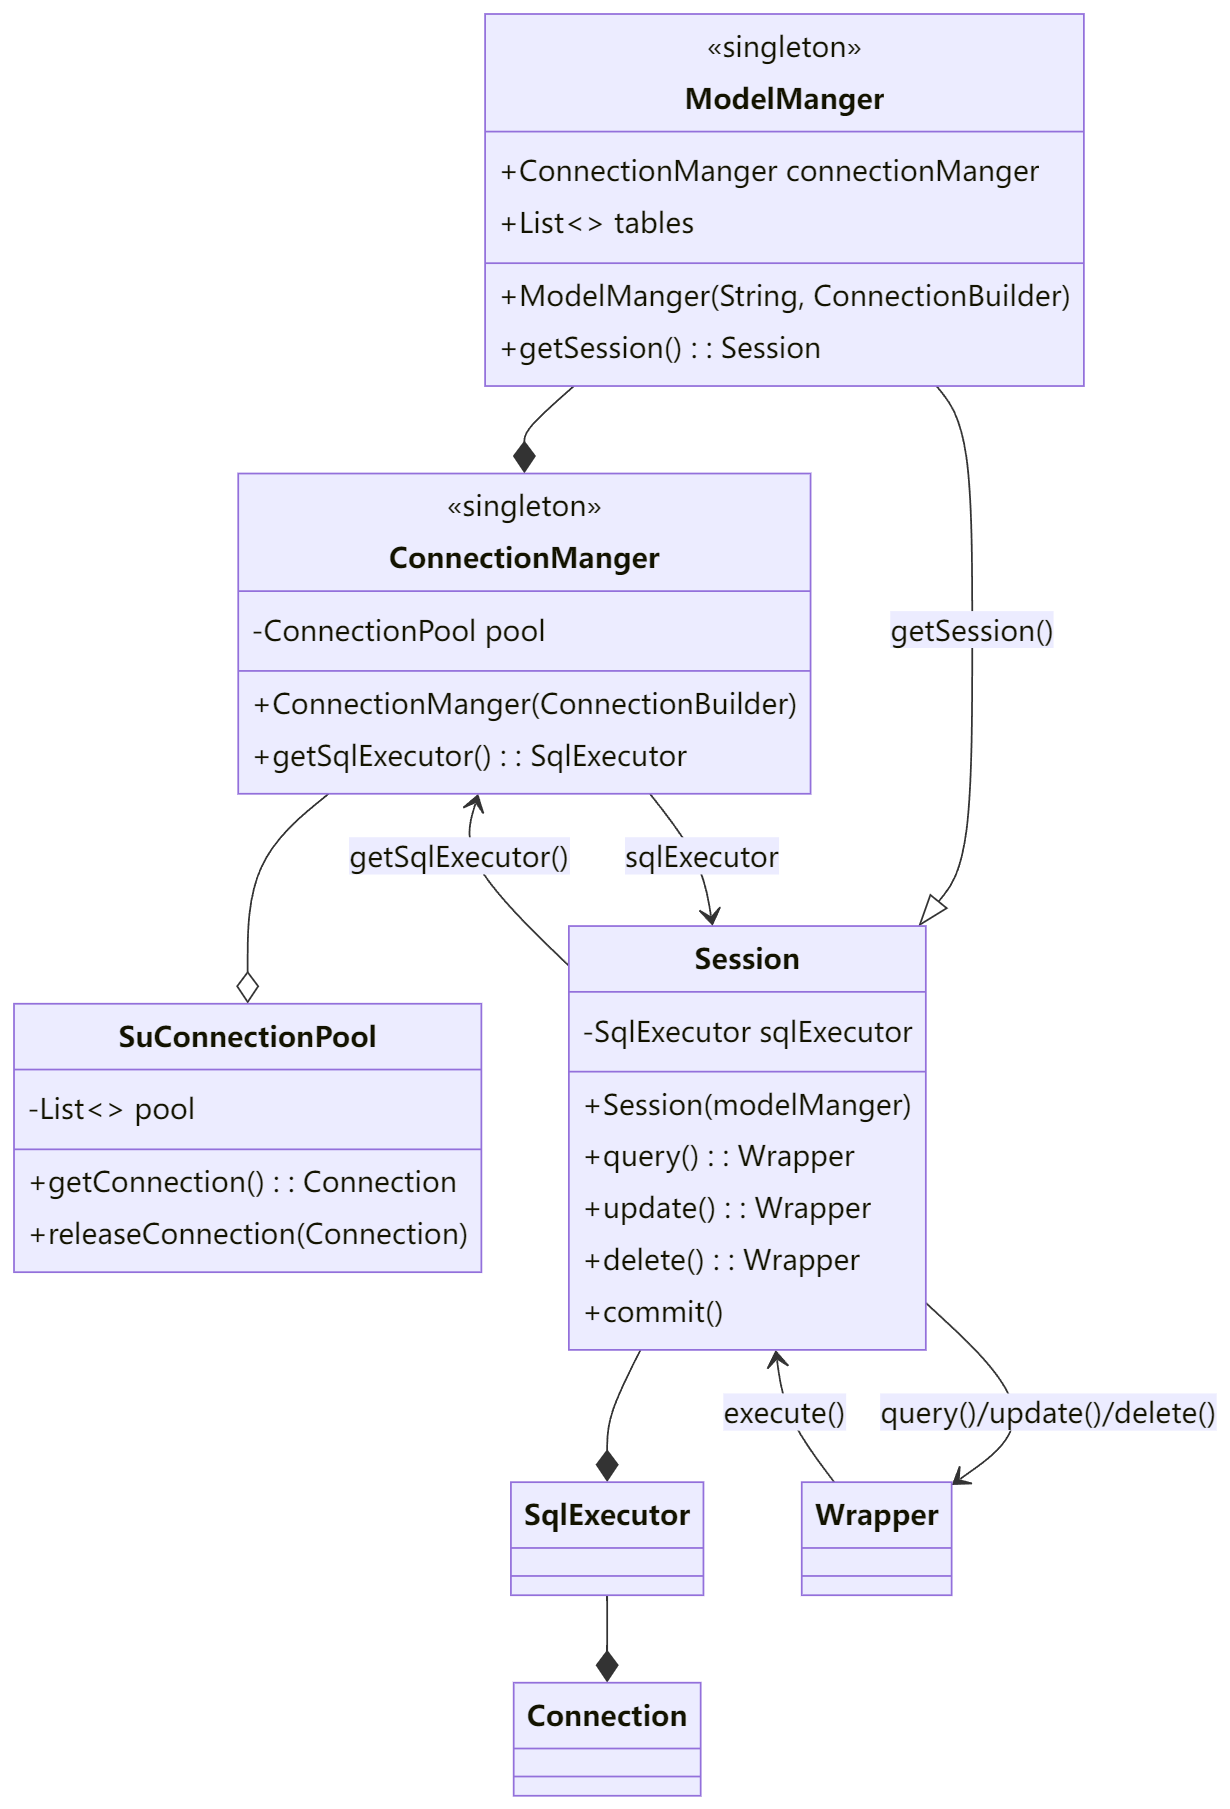
\includegraphics[height=\textheight]{assets/171437405179013.png}


    \end{figure}
  \end{minipage}%\hspace{0.1cm}

\end{frame}





\begin{frame}{IOC/DI/AOP}


  \begin{itemize}
    \item
          支持对象的生命周期管理,构建时自动注入需要的参数,销毁时调用destroy方法优雅的释放占用的资源。
    \item
          支持构造器注入,自动构建构造方法需要的对象,如果有嵌套则递归构建。
    \item
          支持AOP编程,支持在构造对象时注入被代理的对象,在不修改原来代码的情况下,在调用对象的方法的时候插入新的逻辑。以此为基础实现了rbac权限认证和统一的审批系统以及声明式事务和锁。
    \item 使用注解优化上述过程,使得代码更加优雅。
  \end{itemize}

\end{frame}




\begin{frame}{RBAC权限认证}

  使用基于AOP的带有分组拓展的RBAC权限认证系统。

  \begin{itemize}
    \item
          权限认证整体框架基于RBAC,给不同的用户分配不同的角色。为了更好的应对群组关系,个人在rbac的基础上拓展了分组系统,用户将会被分配一个带有分组的角色,该角色只有操作分组内资源的的权限。
    \item
          基于AOP,在方法被执行之前自动使用用户身份和用户的角色进行权限校验,无需在方法内部添加额外的代码。
  \end{itemize}
\end{frame}


\begin{frame}{审批系统}


  基于AOP实现统一的审批系统,无需更改接口即可将旧接口改为需要审批。\\
  实现原理:

  \begin{itemize}
    \item
          在权限校验的时候设置断点,记录请求的方法和参数,保存请求的原因后直接返回,告知用户请求已提交,等待审批
    \item
          给审批人发送通知,审批人可以看到请求的原因,审批通过后,再执行操作
    \item
          审批的消息带有一个回调地址,审批通过,前端调用回调地址,后端执行操作
    \item
          通过请求的方法和参数,再次调用一次请求,但是这次不会再次进入权限校验,直接执行操作,不会再走请求流程
  \end{itemize}

\end{frame}





\begin{frame}{子钱包设计}

  \begin{itemize}
    \item
          群组给用户分配资金,抽象为用户获得群组子钱包,子钱包同为钱包,可以正常与其他账户进行交易。

  \end{itemize}

\end{frame}




\begin{frame}{声明式事务和锁}
  \begin{minipage}{0.4\linewidth}
    一行注解,即可给当前方法开启事务或锁
  \end{minipage}\hspace{0.3cm}
  \begin{minipage}{0.45\linewidth}
    \begin{figure}[h]
      \centering
      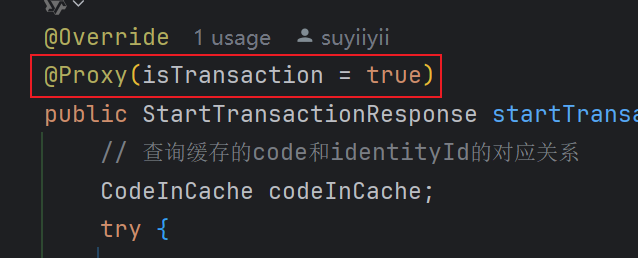
\includegraphics[height=.4\textheight]{assets/image-20240429091843971.png}

    \end{figure}
  \end{minipage}%\hspace{0.1cm}

\end{frame}




\begin{frame}{交易协议}
  基于开放共赢的理念,我设计了一套开放的通用的跨平台的交易api,在保证交易安全的前提下可以实现跨多平台的安全互信,为平台发展提供了更多可能性。
  \begin{itemize}
    \item
          用户网上购物,下订单后网页弹出二维码,用户使用铛铛支付扫描二维码直接提示金额,身份认证通过后付款
    \item
          项目作者在宿舍门口卖炒粉,贴一张收款码在门口,用户使用铛铛支付扫描收款码,手动输入金额,身份认证通过后付款
    \item
          用户去超市购物,收银员输入金额,用户使用铛铛支付,在身份认证之后出示付款码,收银员扫描付款码,此时不需要身份验证,直接付款
  \end{itemize}
\end{frame}





\begin{frame}{交易协议}
  网上购物场景
  \begin{minipage}{0.45\linewidth}
    \begin{figure}[h]
      \centering
      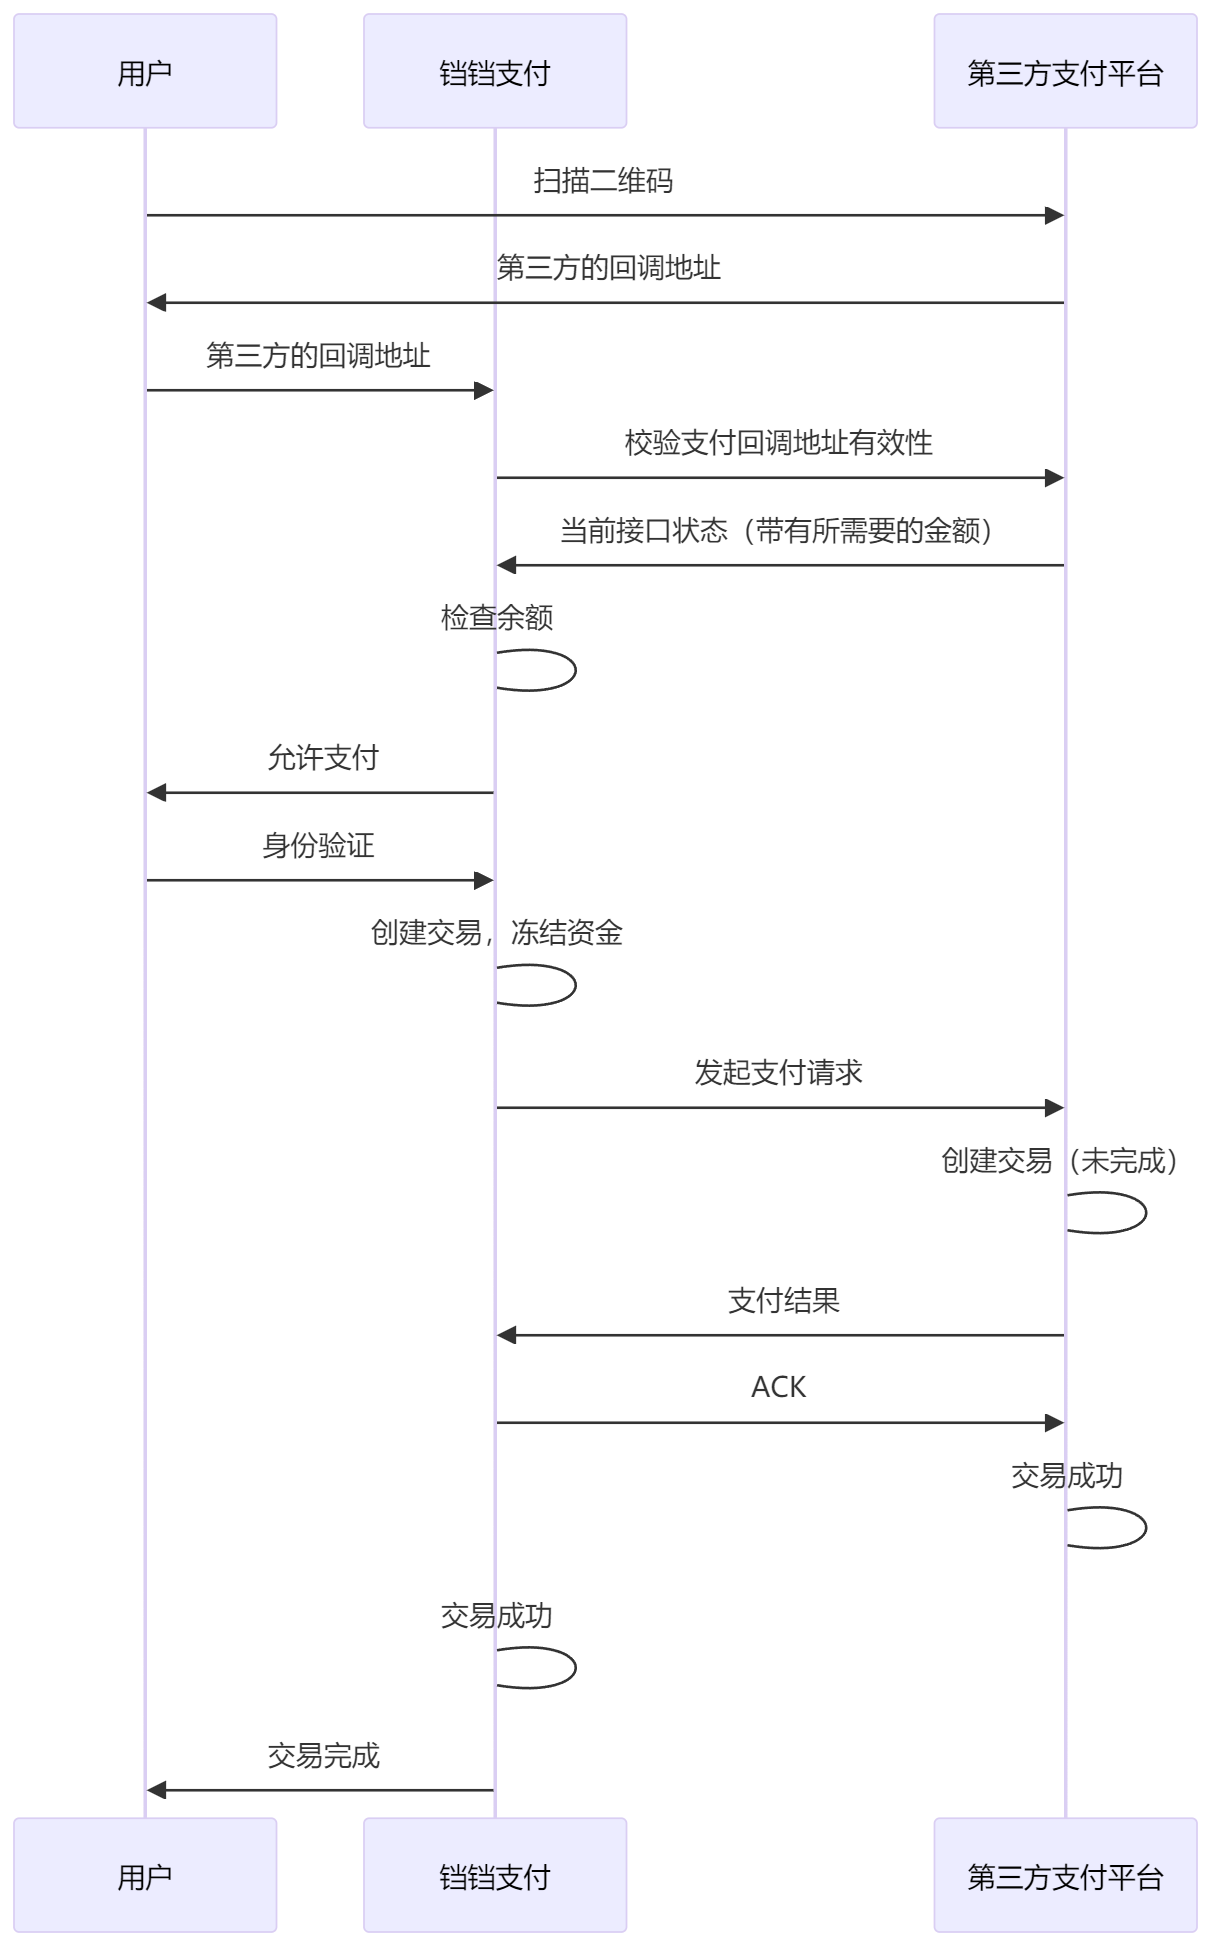
\includegraphics[height=\textheight]{assets/171437647446218.png}

    \end{figure}
  \end{minipage}%\hspace{0.1cm}

\end{frame}



\section{项目开发亮点}

\begin{frame}{应用程序的无状态}
  简单介绍架构演进过程
\end{frame}



\begin{frame}{原始的单体架构}
  \begin{minipage}{0.4\linewidth}
    应用服务器需要处理客户端的各种请求,可能需要长期保存文件或者临时保存文件,一般数据库会独立出来部署到其他地方,但是其他数据一般都会保存在本地。
  \end{minipage}\hspace{0.3cm}
  \begin{minipage}{0.45\linewidth}
    \begin{figure}[h]
      \centering
      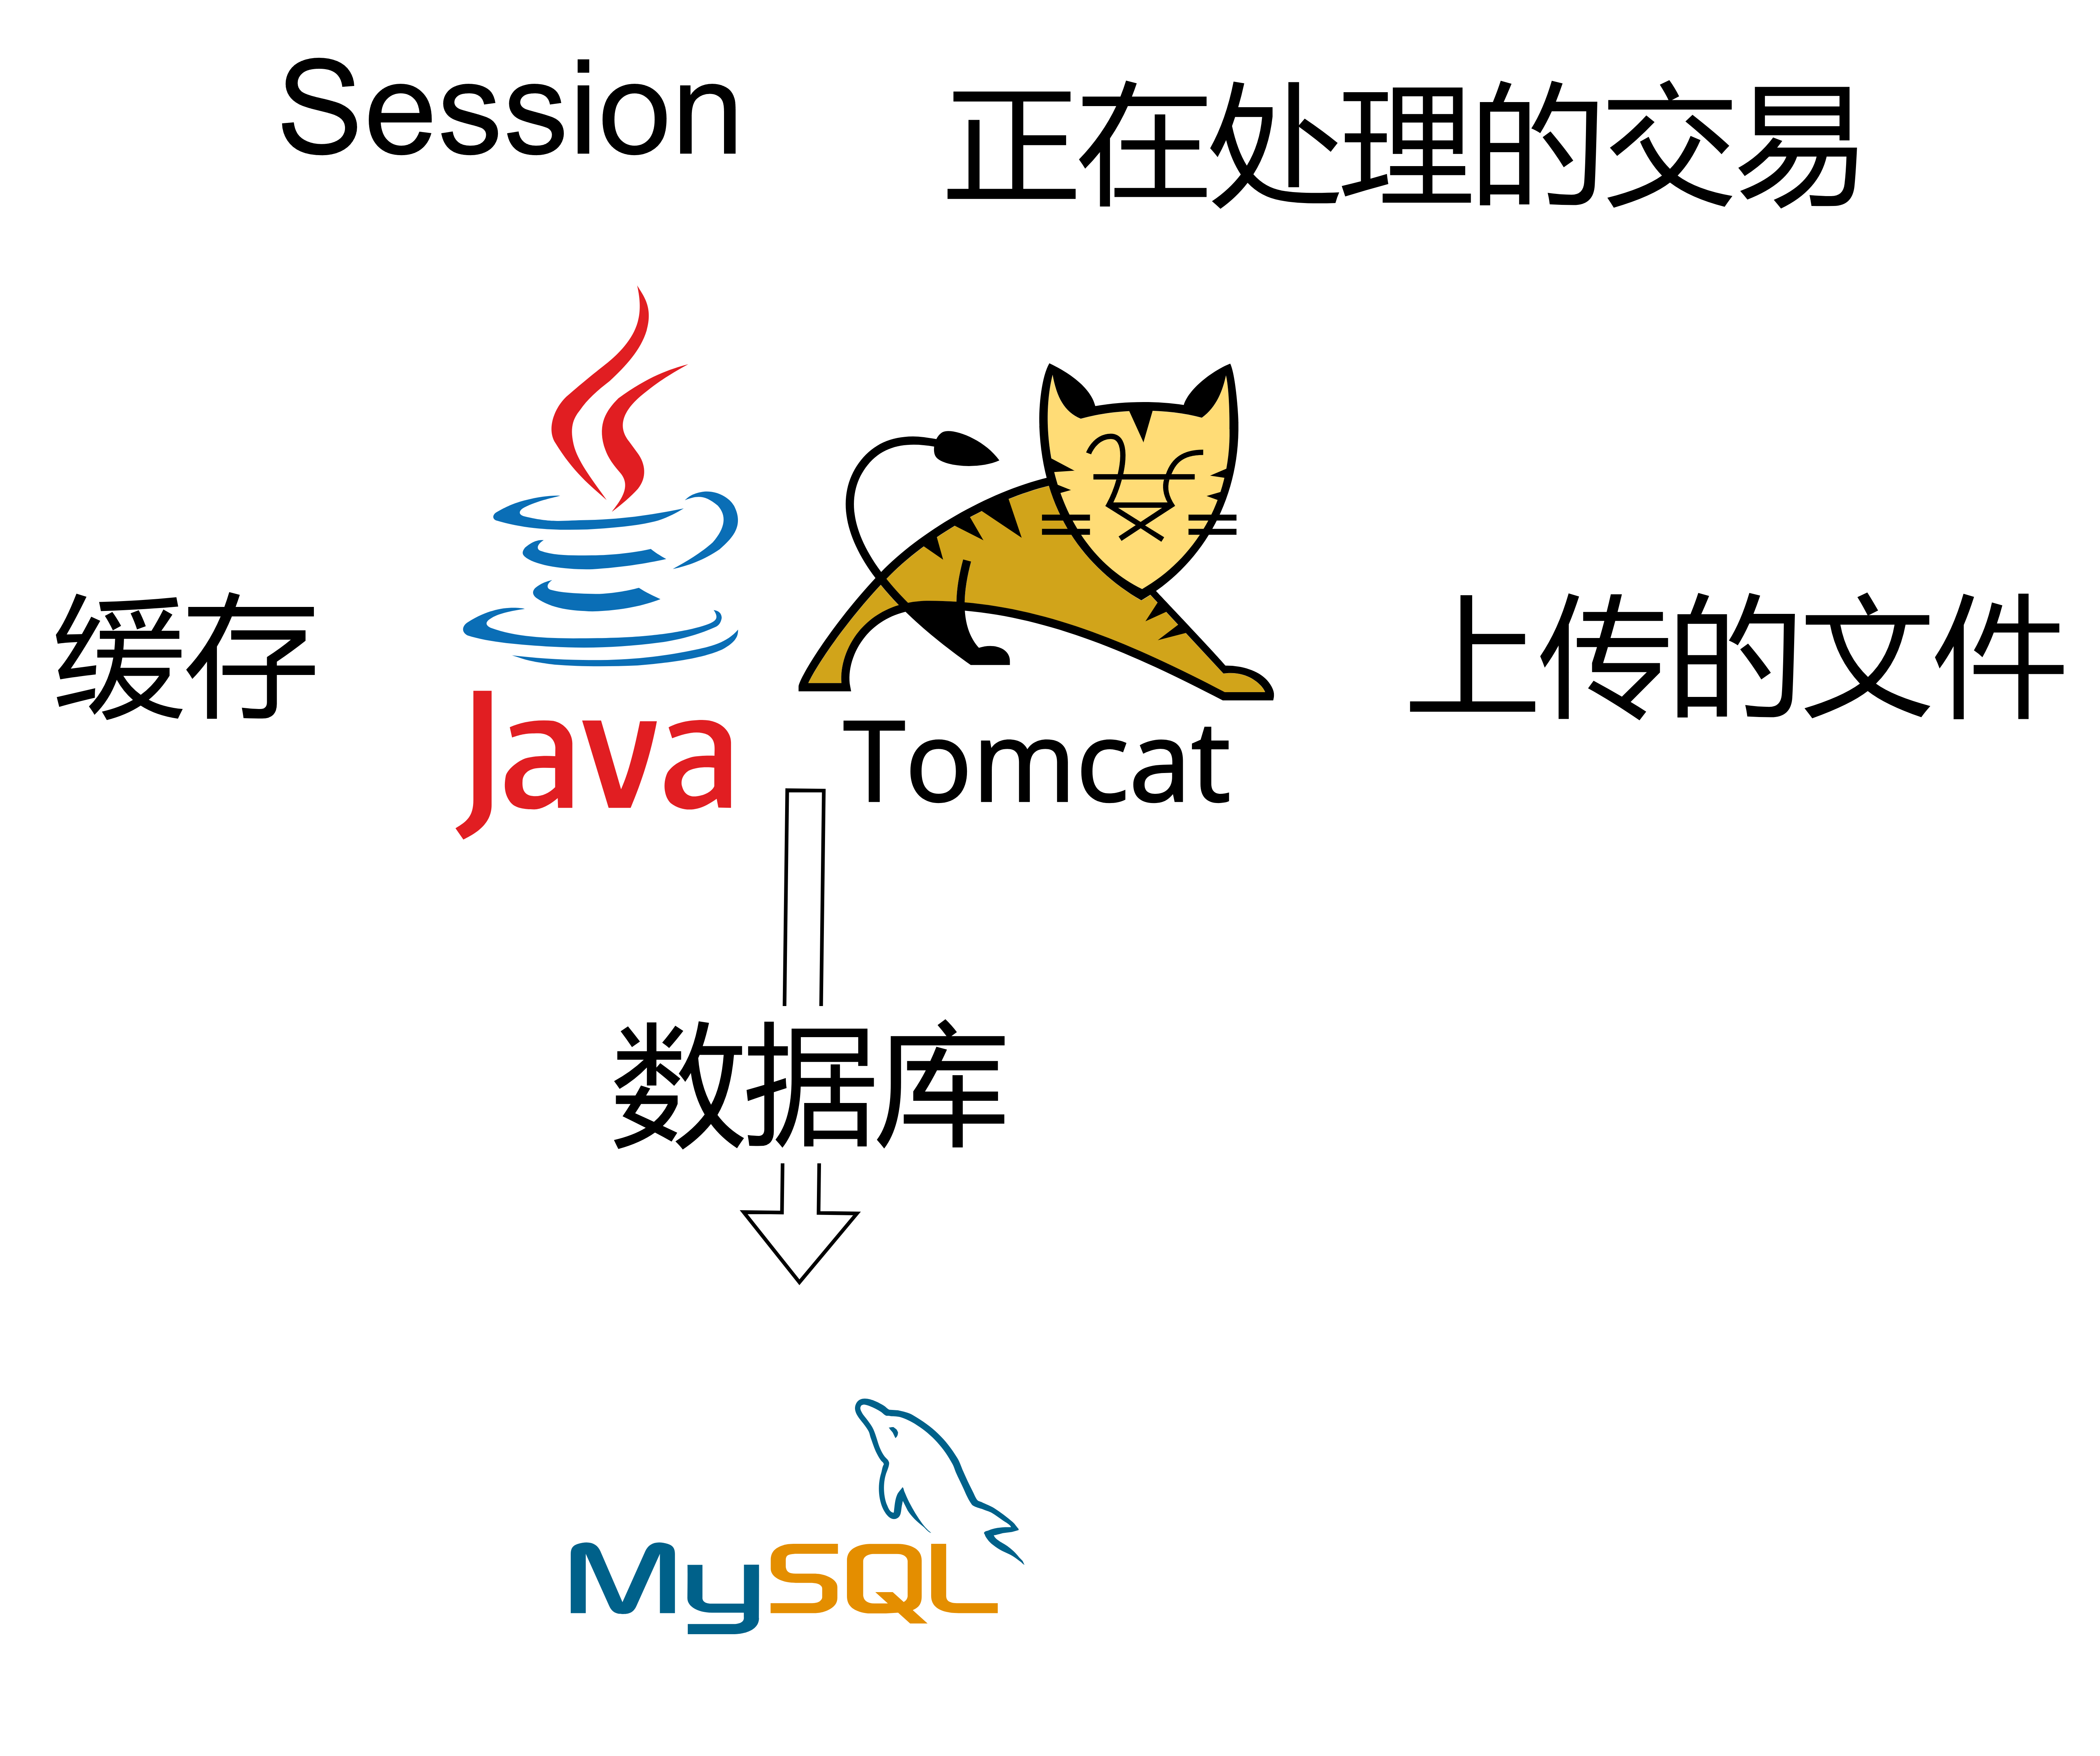
\includegraphics[height=0.8\textheight]{assets/下载.png}

    \end{figure}
  \end{minipage}%\hspace{0.1cm}

\end{frame}




\begin{frame}{职能外包}
  \begin{minipage}{0.4\linewidth}
    可以将不同的功能转移给专用的中间件进行处理,可以讲应用本体无状态化。
  \end{minipage}\hspace{0.3cm}
  \begin{minipage}{0.45\linewidth}
    \begin{figure}[h]
      \centering
      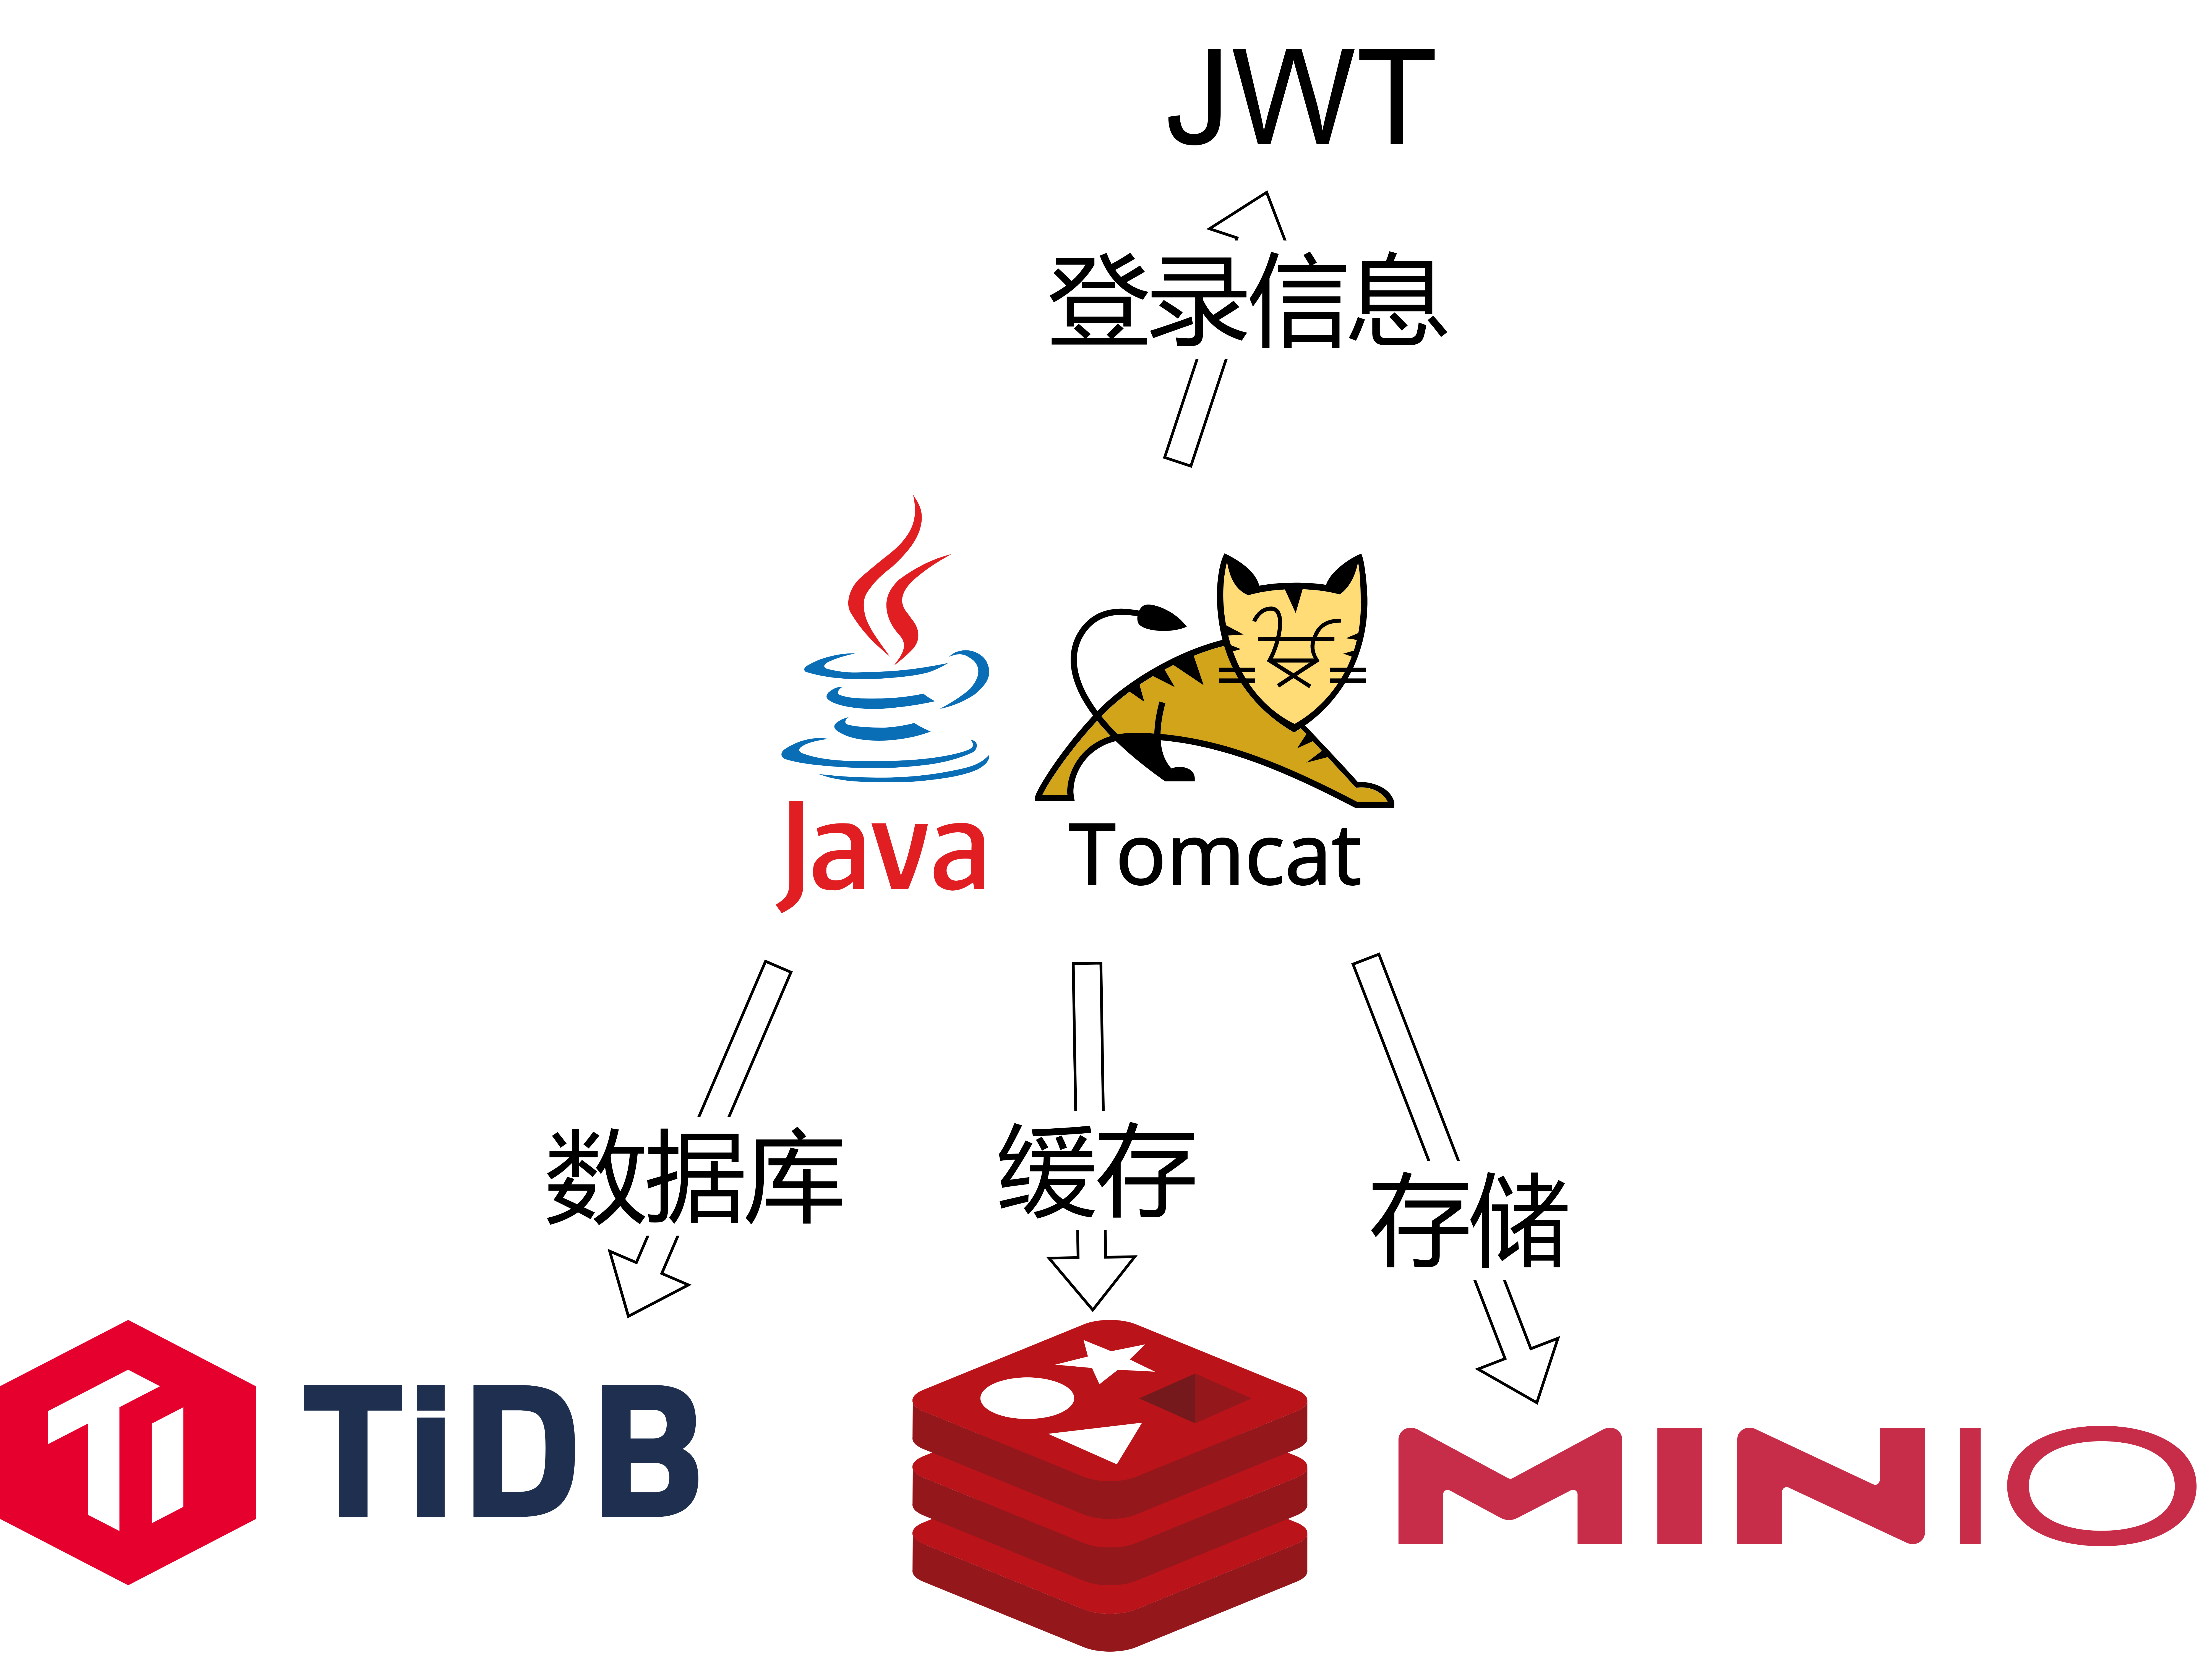
\includegraphics[height=0.8\textheight]{assets/未命名绘图.drawio (1).png}

    \end{figure}
  \end{minipage}%\hspace{0.1cm}
\end{frame}




\begin{frame}{职能外包}
  \begin{minipage}{0.4\linewidth}
    由于应用服务器不再需要本地存储数据,所以可以将应用服务器打包成容器镜像。
  \end{minipage}\hspace{0.3cm}
  \begin{minipage}{0.45\linewidth}
    \begin{figure}[h]
      \centering
      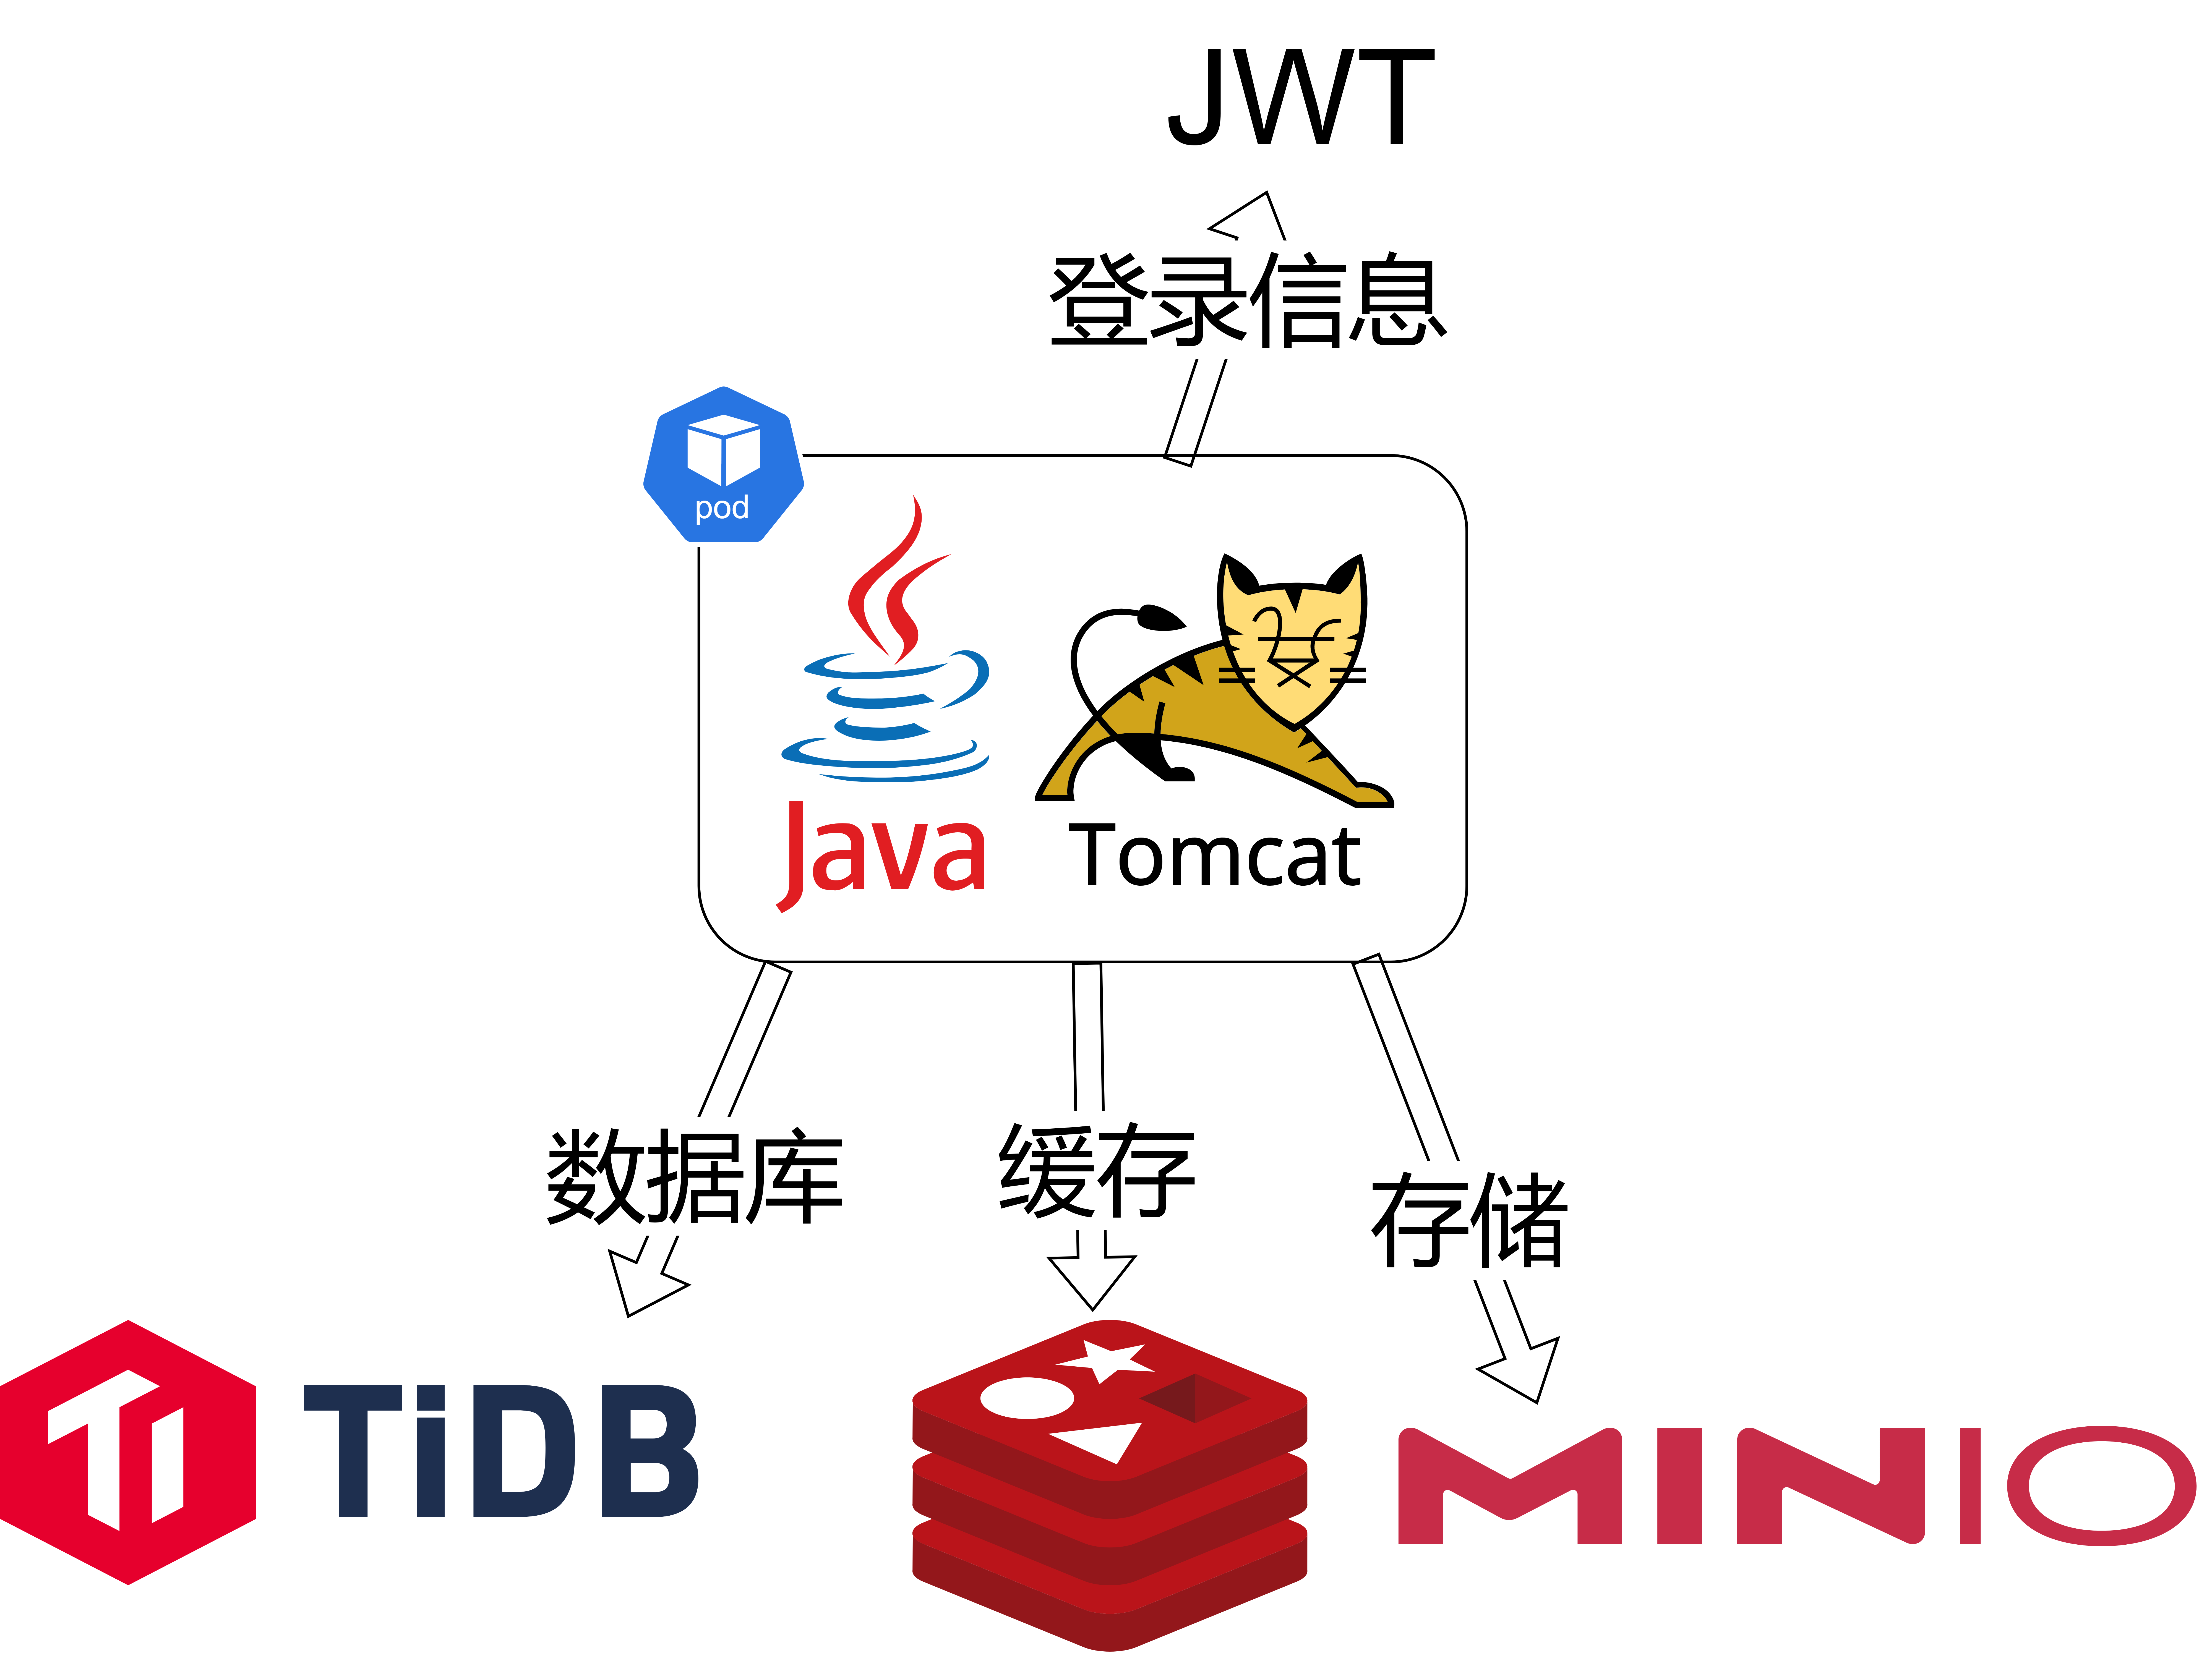
\includegraphics[height=0.8\textheight]{assets/未命名绘图.drawio (2).png}

    \end{figure}
  \end{minipage}%\hspace{0.1cm}

\end{frame}



\begin{frame}{集群部署}
  \begin{minipage}{0.4\linewidth}
    应用保持无状态后并使用容器打包后,便可以很方便的横向扩容,可以使用编排平台进行集群部署。
  \end{minipage}\hspace{0.3cm}
  \begin{minipage}{0.45\linewidth}
    \begin{figure}[h]
      \centering
      \includegraphics[height=0.8\textheight]{assets/未命名绘图.drawio (3).png}

    \end{figure}
  \end{minipage}%\hspace{0.1cm}

\end{frame}


\begin{frame}{项目架构}

  \subparagraph{应用}\label{ux5e94ux7528}

  \begin{itemize}
    \item
          应用使用tomcat容器为基础,容器化部署。
  \end{itemize}

  \subparagraph{中间件}\label{ux4e2dux95f4ux4ef6}

  \begin{itemize}
    \item
          \textbf{TiDB} 数据库中间件,提供结构化数据存储的能力,以兼容
          \texttt{mysql\ 8.0}
          的接口的形式提供服务,用于存储平台产生的绝大多数数据。
    \item
          \textbf{Redis}
          缓存中间件,提供快速的的内存kv数据库的能力,用于临时存储邮箱验证码,交易凭据等临时数据。
    \item
          \textbf{MinIO}
          存储中间件,提供高效存储非结构化数据的能力,用户存储用户上传的头像等二进制文件,以\texttt{S3}兼容接口的形式提供。
  \end{itemize}

  \subparagraph{负载均衡}\label{ux8d1fux8f7dux5747ux8861}

  \begin{itemize}
    \item
          \textbf{traefik} 网络路由中间件,为集群提供负载均衡功能。
  \end{itemize}

  \subparagraph{容器编排}\label{ux5bb9ux5668ux7f16ux6392}

  \begin{itemize}
    \item
          \textbf{Kubernetes}
          容器编排平台,它提供了容器编排等能力。
  \end{itemize}

\end{frame}



\begin{frame}{项目架构}

  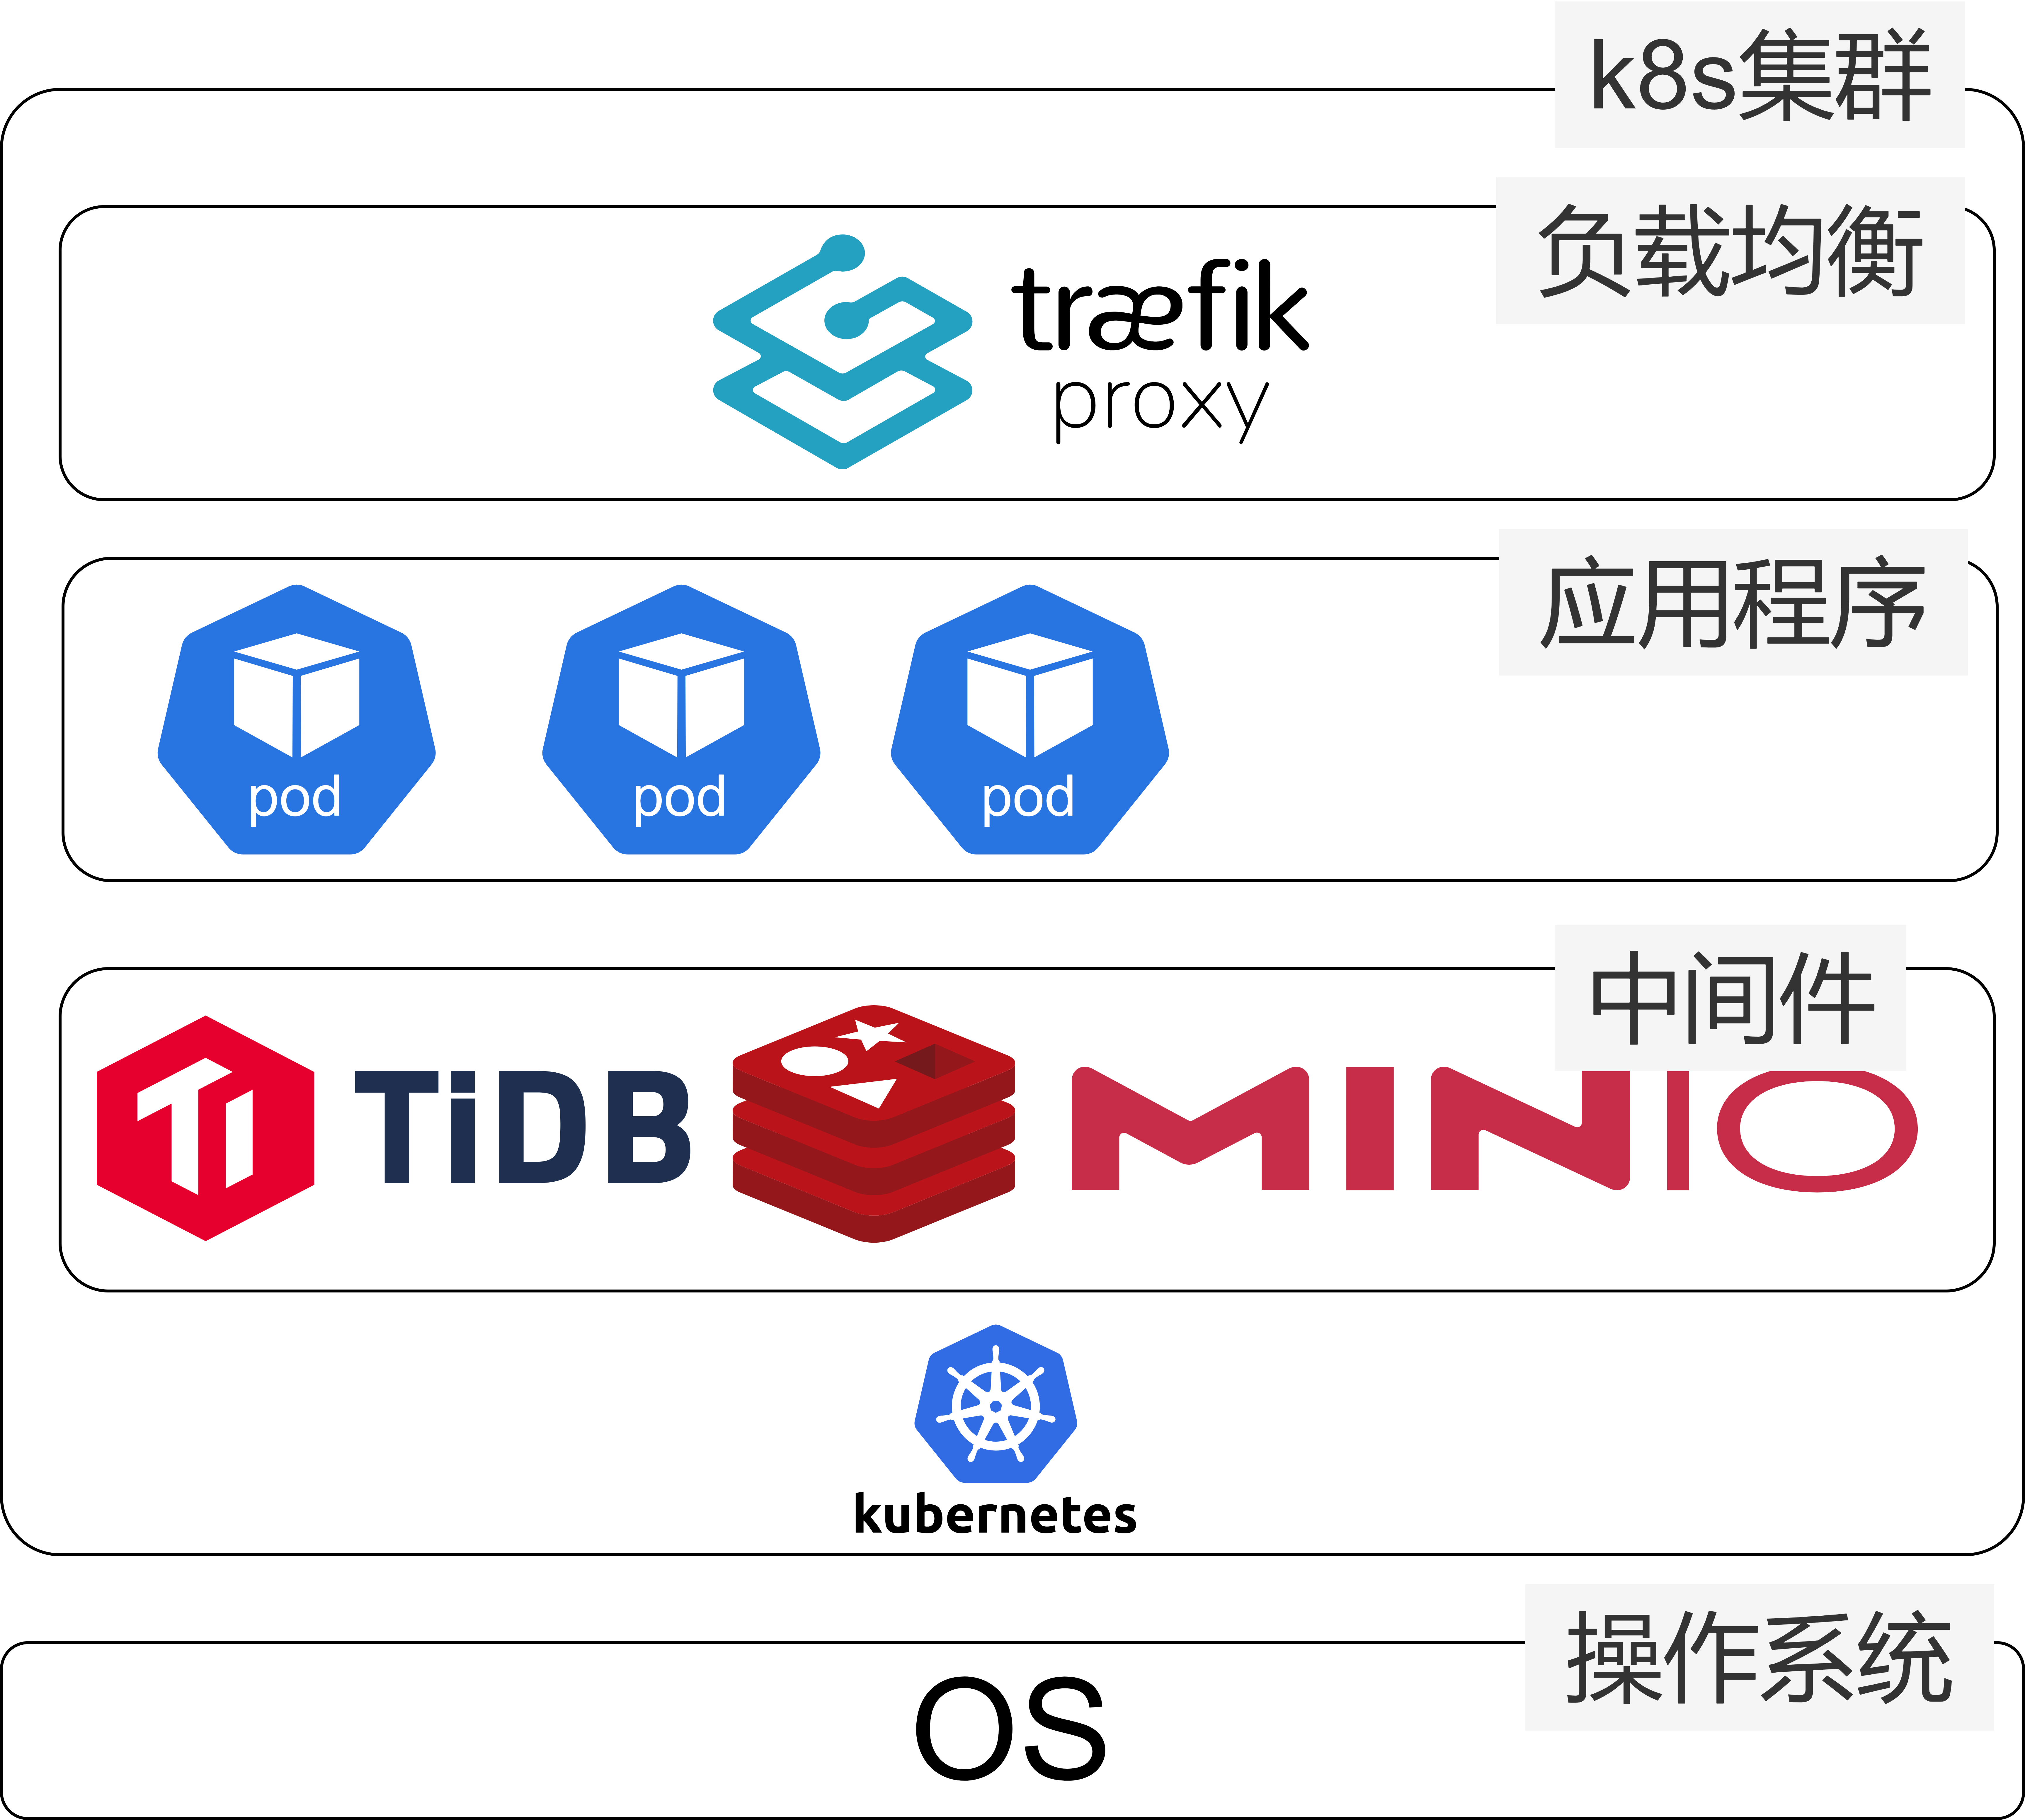
\includegraphics[height=0.8\textheight]{assets/导出 (1).png}


\end{frame}




\begin{frame}{GitOps工作流}
  \begin{minipage}{0.4\linewidth}
    项目使用GitOps工作流,程序运行环境也使用代码定义,实现基础架构即代码(IaC) ,从而将基础架构的配置和管理自动化,提高了开发效率和系统可靠性。同时,GitOps工作流还提供了版本控制和回退机制,确保了系统的稳定性和可追溯性。
  \end{minipage}\hspace{0.3cm}
  \begin{minipage}{0.45\linewidth}
    \begin{figure}[h]
      \centering
      \includegraphics[height=0.8\textheight]{assets/导出 (2).png}

    \end{figure}
  \end{minipage}%\hspace{0.1cm}

\end{frame}



\section{项目功能亮点}

\begin{frame}{全局审计日志}
  \begin{minipage}{0.4\linewidth}
    系统在做权限认证的同时会记录用户信息以及认证结果和请求相关信息并存储到数据库中,可以分析用户行为,识别恶意请求。
  \end{minipage}\hspace{0.3cm}
  \begin{minipage}{0.45\linewidth}
    \begin{figure}[h]
      \centering
      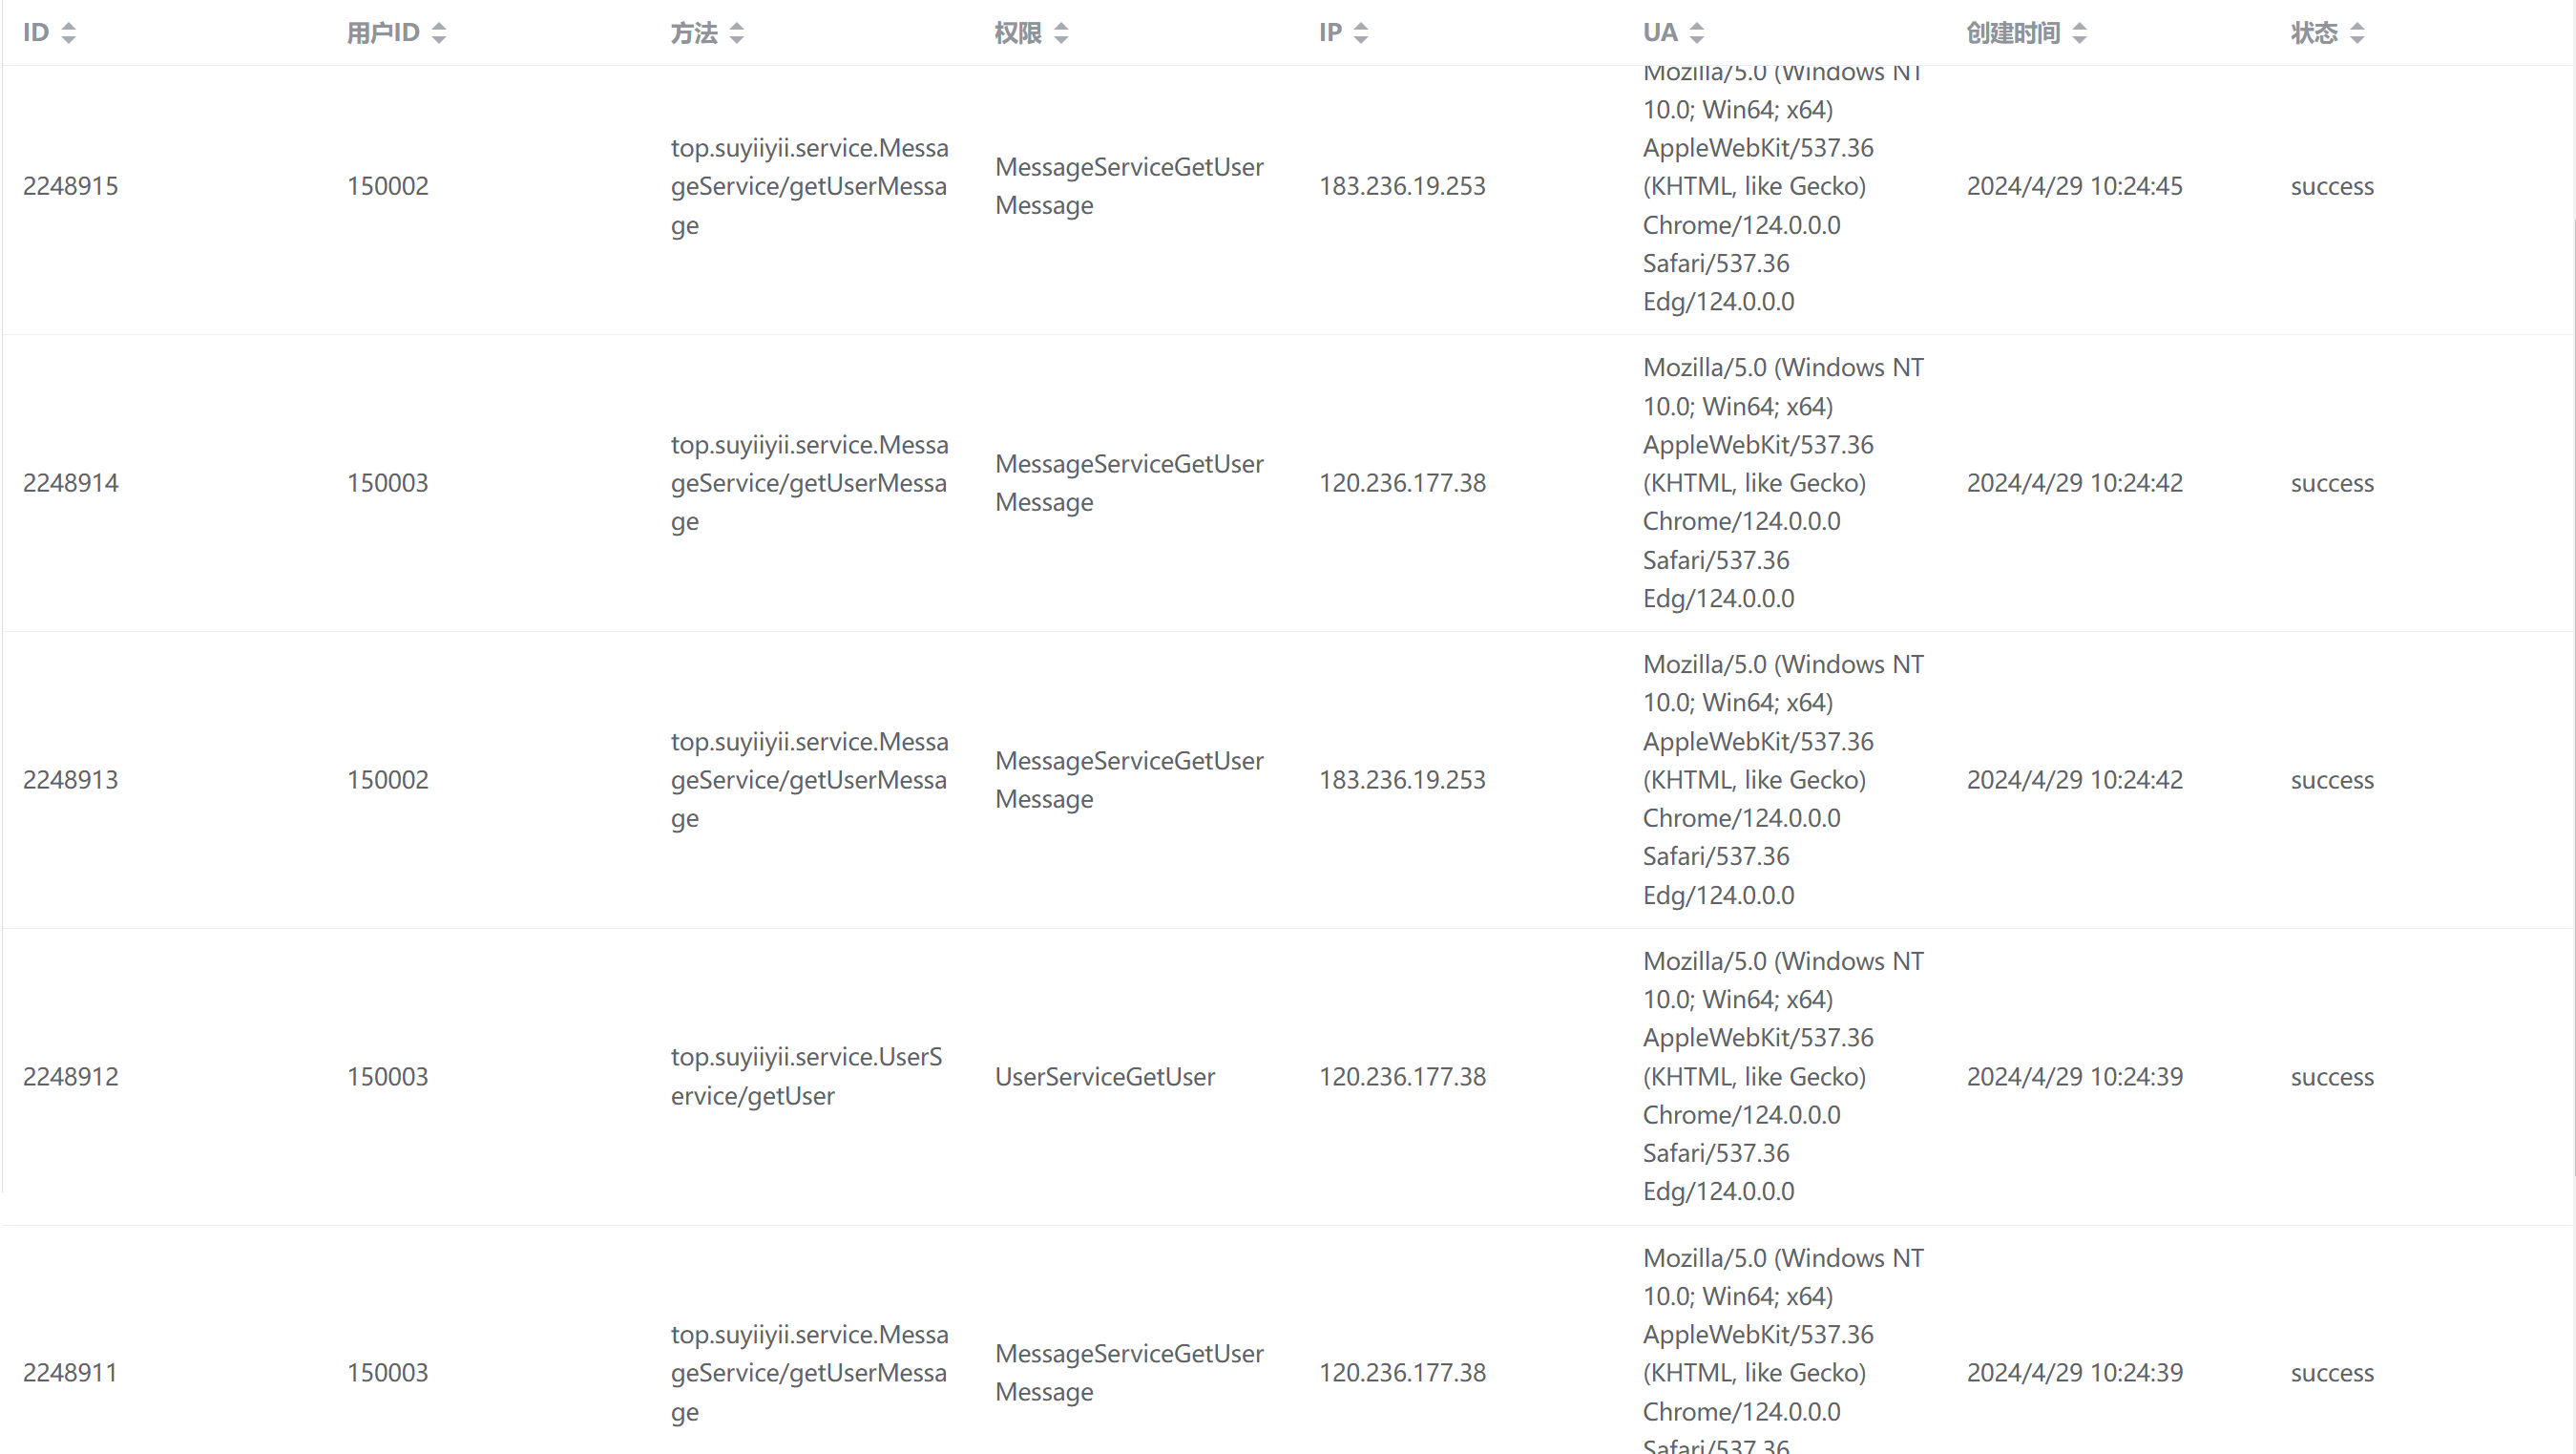
\includegraphics[height=0.8\textheight]{assets/image-20240429120219733.png}

    \end{figure}
  \end{minipage}%\hspace{0.1cm}

\end{frame}





\begin{frame}{HTTPS}
  \begin{minipage}{0.4\linewidth}
    用户请求从浏览器到中转服务器到应用服务器,全程 \texttt{HTTPS/TLS} 加密。
  \end{minipage}\hspace{0.3cm}
  \begin{minipage}{0.45\linewidth}
    \begin{figure}[h]
      \centering
      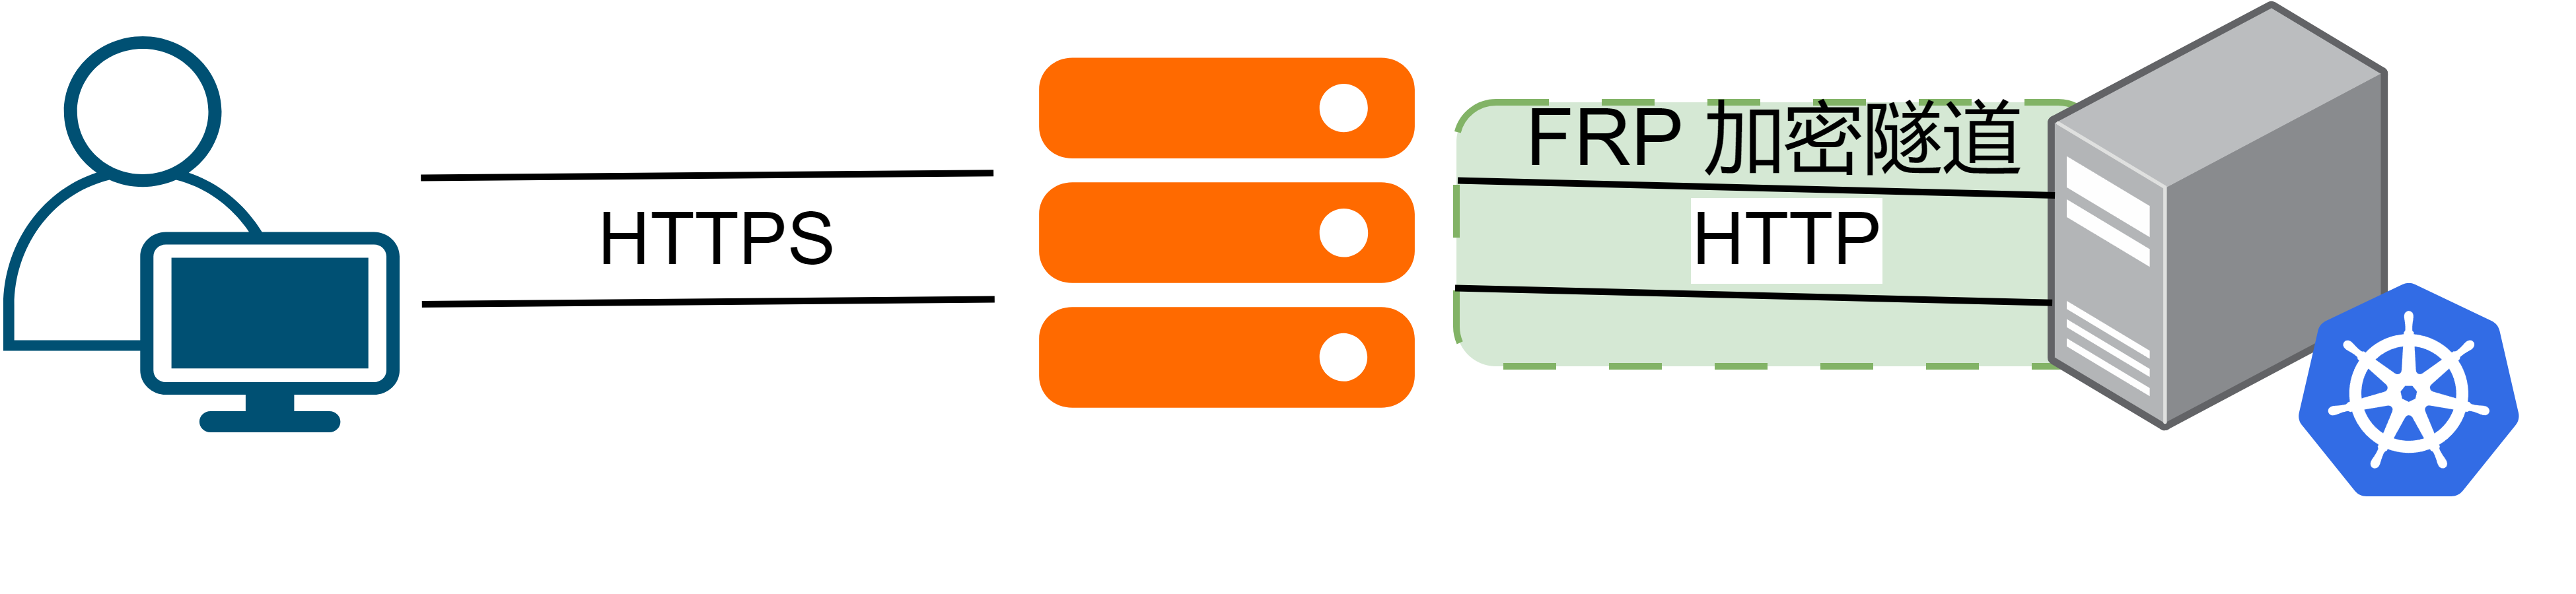
\includegraphics[width=1.3\textwidth]{assets/未命名绘图.drawio (4).png}

    \end{figure}
  \end{minipage}%\hspace{0.1cm}

\end{frame}



\begin{frame}{RSA 签名}
  \begin{minipage}{0.4\linewidth}
    平台之间交互必须使用私钥对请求体进行签名,接收交易请求方将会使用内置的公钥尝试验签,如签名不存在或验签失败,则拒绝响应。
  \end{minipage}\hspace{0.3cm}
  \begin{minipage}{0.45\linewidth}
    \begin{figure}[h]
      \centering
      \includegraphics[width=1.3\textwidth]{assets/未命名绘图.drawio (5).png}

    \end{figure}
  \end{minipage}%\hspace{0.1cm}

\end{frame}


\begin{frame}{二维码支付}
  \begin{minipage}{0.4\linewidth}
    平台支持扫描二维码和生成二维码,极大的提高了支付的便利性。
  \end{minipage}\hspace{0.3cm}
  \begin{minipage}{0.45\linewidth}
    \begin{figure}[h]
      \centering
      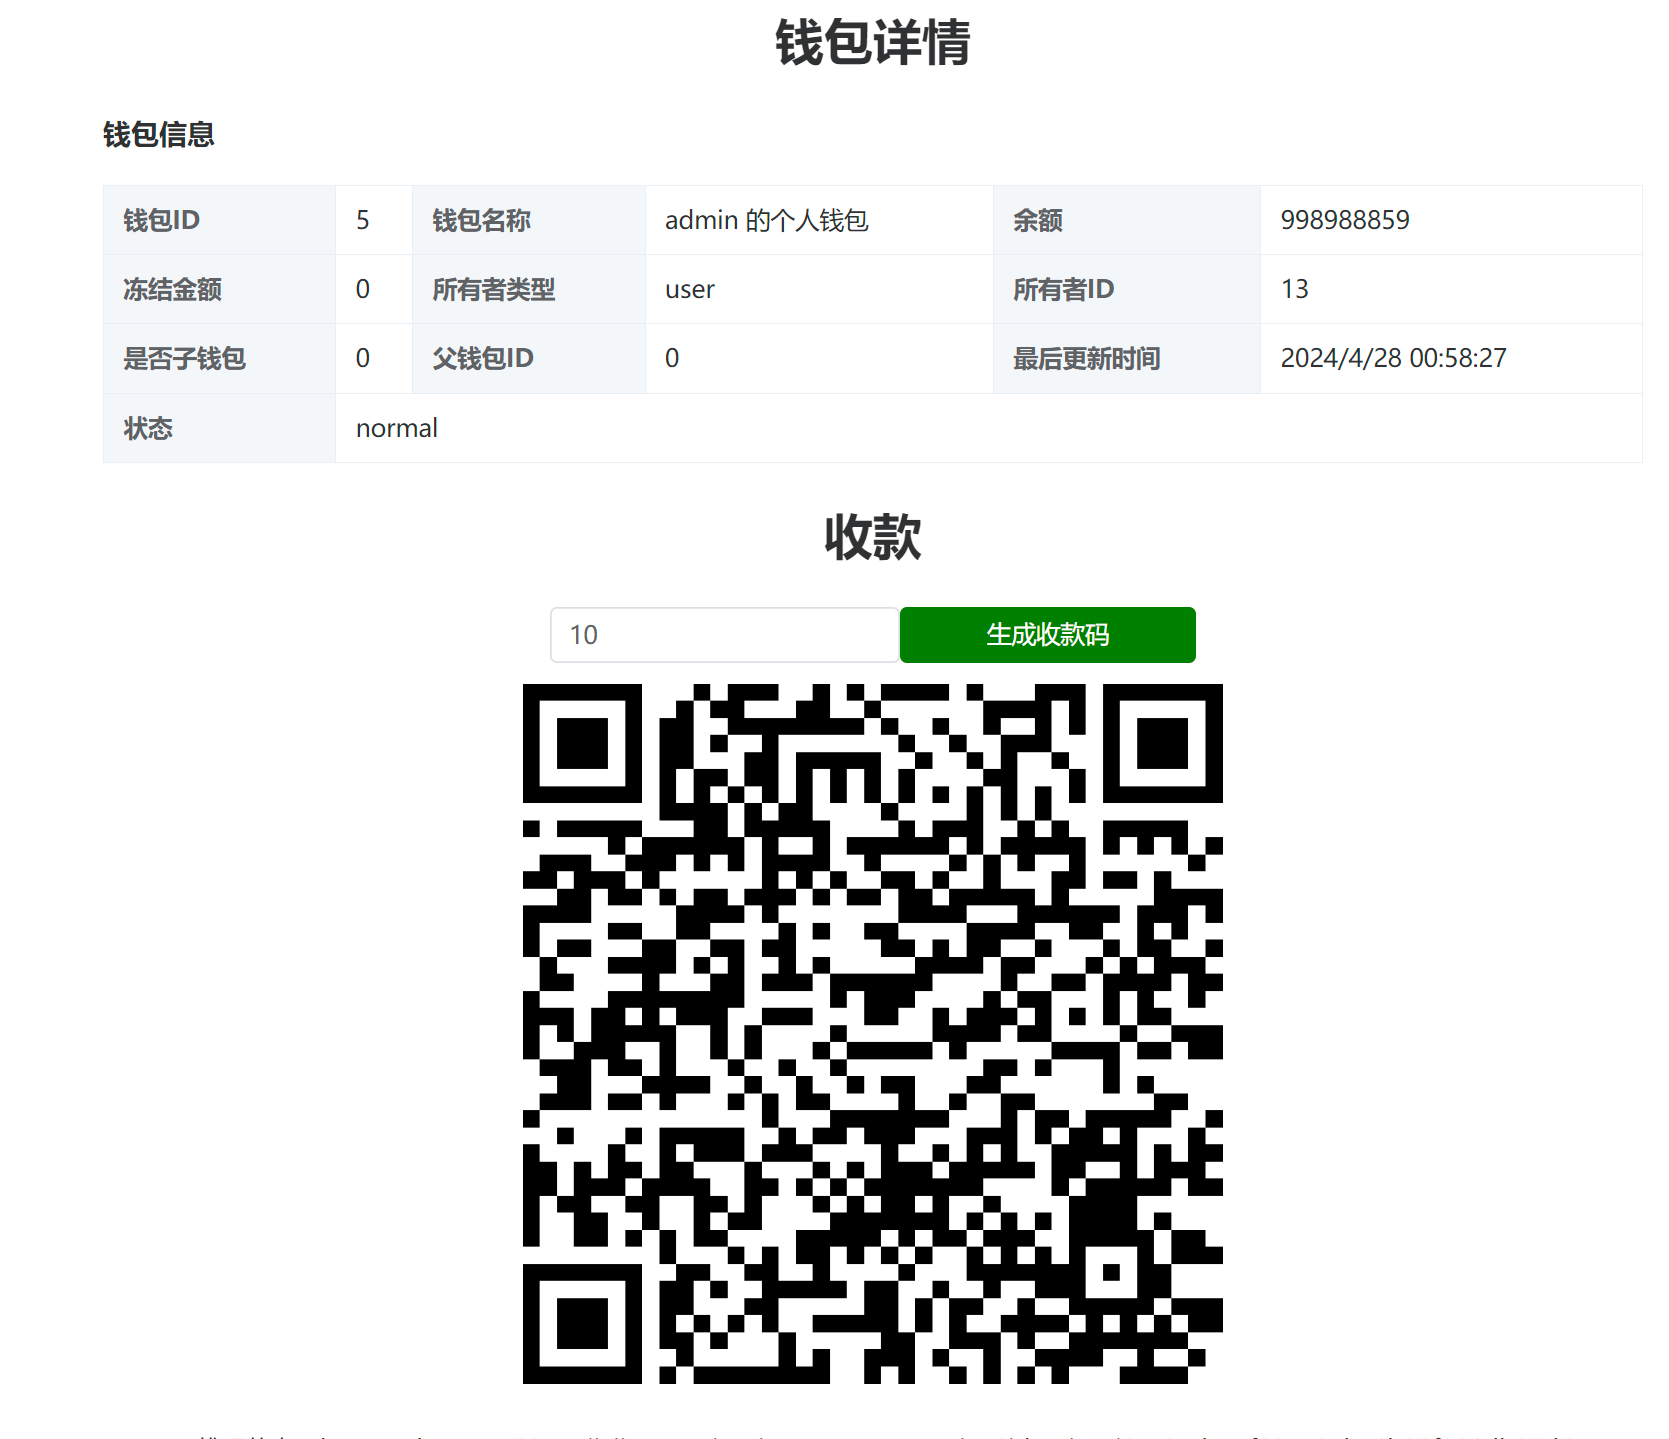
\includegraphics[height=0.8\textheight]{assets/image-20240429092620969.png}

    \end{figure}
  \end{minipage}%\hspace{0.1cm}

\end{frame}

\begin{frame}{还有亿些项目亮点}
  \begin{itemize}
    \item
          邮箱验证码
    \item
          人机验证码
    \item
          Jwt做登录状态
    \item
          支持用户上传自己的头像和文件
    \item
          全程日志记录
    \item
          全自动参数校验
    \item
          统一异常处理
    \item
          使用Apifox记录接口信息
    \item
          抵御Sql注入、Xss攻击
    \item
          数据库用户密码加盐存储
    \item
          Git 使用双分支开发,dev分支定时合并到主分支
    \item
          Git提交粒度小
    \item
          \ldots\ldots{}
  \end{itemize}
\end{frame}

%------------------------------------------------




% %------------------------------------------------

% \begin{frame}
%   \frametitle{设计思路}
%   \begin{block}{Slides with \LaTeX}
%     Beamer offers a lot of functions to create nice slides using \LaTeX.
%   \end{block}

%   \begin{block}{The basis}
%     内部使用以下主题
%     \begin{itemize}
%       \item split
%       \item whale
%       \item rounded
%       \item orchid
%     \end{itemize}
%   \end{block}
% \end{frame}
% %------------------------------------------------
% \begin{frame}
%   \frametitle{带数字列表}
%   \begin{enumerate}
%     \item This just shows the effect of the style
%     \item It is not a Beamer tutorial
%     \item Read the Beamer manual for more help
%     \item Contact me only concerning the style file
%   \end{enumerate}
% \end{frame}
% %------------------------------------------------
% \begin{frame}{块并列}
%   \begin{columns}
%     \begin{column}{0.5\textwidth}
%       \begin{block}{block1}
%         %\footnotesize{
%         \begin{enumerate}
%           \item item1
%                 \begin{itemize}
%                   \item  item1.1
%                 \end{itemize}
%           \item item2
%                 \begin{itemize}
%                   \item item2.1
%                 \end{itemize}
%           \item item3
%                 \begin{itemize}
%                   \item item3.1
%                 \end{itemize}
%         \end{enumerate}
%         %}    
%       \end{block}
%     \end{column}
%     \begin{column}{0.5\textwidth}
%       \begin{block}{block2}
%         %\footnotesize{
%         \begin{enumerate}
%           \item item1
%                 \begin{itemize}
%                   \item  item1.1
%                 \end{itemize}
%           \item item2
%                 \begin{itemize}
%                   \item item2.1
%                 \end{itemize}
%           \item item3
%                 \begin{itemize}
%                   \item item3.1
%                 \end{itemize}
%         \end{enumerate}
%         %}    
%       \end{block}
%     \end{column}
%   \end{columns}
% \end{frame}
% %------------------------------------------------

% \begin{frame}{图片}
%   \begin{minipage}{0.4\linewidth}
%     \begin{figure}[h]
%       \centering
%       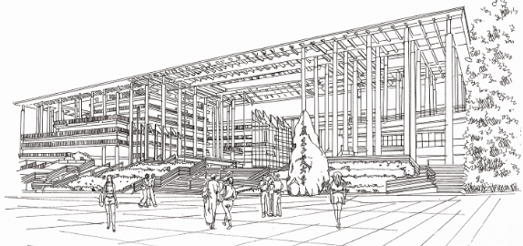
\includegraphics[height=.4\textheight]{res/GDUT-gate.png}
%       \caption{GDUT}
%     \end{figure}
%   \end{minipage}\hspace{0.3cm}
%   \begin{minipage}{0.45\linewidth}
%     \begin{figure}[h]
%       \centering
%       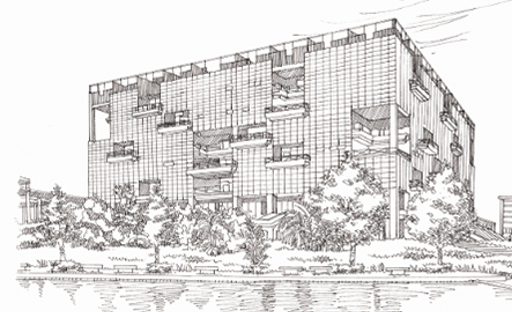
\includegraphics[height=.4\textheight]{res/GDUT-library.png}
%       \caption{GDUT}
%     \end{figure}
%   \end{minipage}%\hspace{0.1cm}
% \end{frame}
% %------------------------------------------------

% \begin{frame}[t]{块中多图}
%   \begin{small}
%     \begin{block}{多图比较与分析}
%       \begin{minipage}{0.5\linewidth}
%         \begin{figure}[h]
%           \centering
%           
\includegraphics[height=.2\textheight]{res/GDUT-logo.png}
%           \caption{GDUT}
%         \end{figure}
%       \end{minipage}\hspace{0.1cm}
%       \begin{minipage}{0.45\linewidth}
%         \begin{figure}[h]
%           \centering
%           
\includegraphics[height=.2\textheight]{res/GDUT-logo_black.png}
%           \caption{GDUT}
%         \end{figure}
%       \end{minipage}\hspace{0.1cm}
%       %\medskip
%       \begin{minipage}{0.5\linewidth}
%         \begin{figure}[h]
%           \centering
%           
\includegraphics[height=.2\textheight]{res/GDUT-logo_white.png}
%           \caption{GDUT}
%         \end{figure}
%       \end{minipage}\hspace{0.4cm}
%       \begin{minipage}{0.4\linewidth}
%         \begin{block}{}
%           \begin{itemize}
%             \scriptsize{
%             \item ****************
%             \item ****************
%             \item ****************
%                   }
%           \end{itemize}
%         \end{block}
%       \end{minipage}
%     \end{block}
%   \end{small}
% \end{frame}
% %------------------------------------------------


% %------------------------------------------------
% \section{结论}
% %------------------------------------------------
% \begin{frame}
%   \subsection{  \frametitle{结论}}

%   \begin{itemize}
%     \item Easy to use
%     \item Good results
%   \end{itemize}
% \end{frame}
% %------------------------------------------------

% %------------------------------------------------
% \section{参考文献}
% %------------------------------------------------
% \begin{frame}
%   \frametitle{参考文献}
%   \begin{block}{}
%     \begin{minipage}{1\linewidth}
%       \scriptsize{
%         \begin{thebibliography}{99} % Beamer does not support BibTeX so references must be inserted manually as below
%           \bibitem{1} R. Sun, Y. Wang, L. Lyu, N. Cheng, S. Zhang, T. Yang, and X.Shen,“Delay-oriented caching strategies in d2d mobile networks,” \emph{IEEE Trans. Veh. Technol.}, vol. 69, no. 8, pp. 8529–8541, Aug. 2020.
%           \item Z. Su, Y. Hui, Q. Xu, T. Yang, J. Liu, and Y. Jia,“An edge caching scheme to distribute content in vehicular networks,” \emph{IEEE Trans. Veh. Technol.}, vol. 67, no. 6, pp. 5346–5356, Jun. 2018.
%           \item Q. Xu, Z. Su, Y. Wang, and K. Zhang,“Secure edge caching for layered multimedia contents in heterogeneous networks,” in \emph{Proc. IEEE Global Commun. Conf.}, Waikoloa, HI, USA, Dec. 2019, pp. 1–6.
%           \item B. Hu, L. Fang, X. Cheng, and L. Yang,“In-vehicle caching (iv-cache) via dynamic distributed storage relay ($d^2$sr) in vehicular networks,” \emph{IEEE Trans. Veh. Technol.}, vol. 68, no. 1, pp. 843–855, Jan. 2019.
%           \item C. Liu, K. Liu, S. Guo, R. Xie, V. C. S. Lee, and S. H. Son,“Adaptive offloading for time-critical tasks in heterogeneous internet of vehicles,” \emph{IEEE Internet Things J.}, vol. 7, no. 9, pp. 7999–8011, Sep. 2020.
%           \item J. Chen, H. Wu, P. Yang, F. Lyu, and X. Shen,“Cooperative edge caching with location-based and popular contents for vehicular networks,” \emph{IEEE Trans. Veh. Technol.}, vol. 69, no. 9, pp. 10291-10305, Jun. 2020.
%         \end{thebibliography}
%       }
%     \end{minipage}
%   \end{block}
% \end{frame}
% %------------------------------------------------


% %------------------------------------------------
\section{}

\begin{frame}
  \begin{block}{Ending}
    \Huge{\centerline{\emph{Thanks for Your Attention!}}}
    \Huge{\centerline{\emph{Q \& A ?}}}
  \end{block}

\end{frame}
%------------------------------------------------

\end{document}